%%%%%%%%%%%%%%%%%%%%%%%%%%%%%%%%%%%%%%%%%%%%%%%%%%%%%%%%%%%%%%%%%%%%%%%%%%%%%%%
% documentclass→
\PassOptionsToPackage{full}{textcomp}
\documentclass[a4paper, twoside, nobib]{tufte-book}
\hypersetup{colorlinks}

%%%%%%%%%%%%%%%%%%%%%%%%%%%%%%%%%%%%%%%%%%%%%%%%%%%%%%%%%%%%%%%%%%%%%%%%%%%%%%%
% metadata

\title[ML-based precision medicine in ischemic heart disease]{%
    Machine Learning-Based Precision Medicine in Ischemic Heart Disease}
\author[Peter Christoffer Holm]{Peter Christoffer Holm}
\publisher{%
    Graduate School of Health and Medical Sciences
    University of Copenhagen%
}
% ←
%%%%%%%%%%%%%%%%%%%%%%%%%%%%%%%%%%%%%%%%%%%%%%%%%%%%%%%%%%%%%%%%%%%%%%%%%%%%%%%
% biblatex configuration →

\usepackage[%
    style=verbose-note,
    %%%%%%%%%%%%%%%%%%%%%%%%%%%%%%%%%%%%%%%%%%
    isbn=false,
    doi=false,
    eprint=false,
    date=year,
    maxcitenames=2,     % when should "et al." be triggered?
    maxbibnames=4,      % when should "et al." be triggered? (in bib)
    sorting=nty,        % name, title, year
    autocite=footnote,  % put citation in sidenotes 
    citereset=chapter,  % reset citation tracker at each chapter
    citetracker=strict,
    trackfloats=true,
    autopunct=true
]{biblatex}

\DeclareCiteCommand{\cite}
  {\usebibmacro{prenote}}
  {\usebibmacro{citeindex}%
   \usebibmacro{footcite}}
  {\multicitedelim}
  {\usebibmacro{cite:postnote}}

\newcommand{\sidecite}[2][0em]{%
	\unskip\sidenote[][#1]{\cite{#2}}%
}

\renewbibmacro{in:}{}
\addbibresource{assets/pch-thesis.bib}

\DeclareSourcemap{
    \maps[datatype=bibtex]{
        \map{
            \pertype{incollection}
            \step[fieldset=url, null]
            \step[fieldset=urldate, null]
        }
        \map{
            \pertype{article}
            \step[fieldset=url, null]
            \step[fieldset=urldate, null]
        }
        \map{
            \pertype{book}
            \step[fieldset=url, null]
            \step[fieldset=urldate, null]
        }
        \map{
            \pertype{online}
            \step[fieldsource=eprinttype, final=true]
            \step[typesource=online, typetarget=article]
            \step[fieldsource=eprinttype, fieldtarget=journaltitle]
            \step[fieldsource=journaltitle, match={arxiv}, replace={arXiv}]
            \step[fieldset=urldate, null]
        }
        \map{
            \pertype{inproceedings}
            \step[fieldset=publisher, null=true]
            \step[fieldset=url, null=true]
            \step[fieldset=urldate, null=true]
        }
        \map{
            \pertype{manual}
            \step[fieldset=url, null=true]
            \step[fieldset=urldate, null=true]
        }
        \map{
            \step[fieldset=pages, null]
            \step[fieldset=pagetotal, null]
            \step[fieldset=series, null]
            \step[fieldset=issue, null]
            \step[fieldset=volume, null]
            \step[fieldset=number, null]
            \step[fieldset=location, null]
            \step[fieldset=editor, null]
            \step[fieldset=eprint, null]
        }
        \map{
            \step[fieldsource=url, final=true]
            \step[fieldset=verba, origfieldval, final=true]
            \step[
               fieldsource=verba, 
               match=\regexp{\A(https?...)?(www.)?}, 
               replace={}
            ]
        }
    }
}

\DeclareFieldFormat{url}{%
  \mkbibacro{URL}\addcolon\space
  \href{#1}{\nolinkurl{\thefield{verba}}}}

% ←
%%%%%%%%%%%%%%%%%%%%%%%%%%%%%%%%%%%%%%%%%%%%%%%%%%%%%%%%%%%%%%%%%%%%%%%%%%%%%%%
% load packages →

% fonts
\usepackage[T1]{fontenc}

\usepackage[osf, p]{ETbb}  % osf in text, tabular lining figures in math
\usepackage[scaled=.95,type1]{cabin}  % sans serif in style of Gill Sans
\usepackage[libertine, vvarbb]{newtxmath}
\usepackage[scaled=.90]{FiraMono}

% misc
\usepackage{amsmath}
\usepackage{amsfonts}
\usepackage{microtype}
\usepackage{booktabs}
\usepackage[danish, british]{babel}
\usepackage{multirow}
\usepackage{tabularx}
\usepackage{multicol}
\usepackage{makecell}
\usepackage{pdfpages}
\usepackage{bookmark}
\usepackage[export]{adjustbox}
\usepackage{datetime}

\usepackage[mode=match]{siunitx}
\DeclareSIUnit\year{yr}

\usepackage{subcaption}
\captionsetup{font=footnotesize}    

\usepackage{marginfix}
\usepackage{appendix}
\usepackage{twemojis}
\usepackage{cleveref}
\usepackage{pgffor}
\usepackage{relsize}  % easy scaling of fonts
\usepackage{bm}
\usepackage[morefloats=200]{morefloats}

% enumerate
\usepackage[inline]{enumitem}
\renewlist{enumerate*}{enumerate*}{1}
\setlist[enumerate*]{
    label=(\roman*), itemjoin={{; }}, itemjoin*={{; and }}
}

% context aware quotation marks
\usepackage{csquotes}  
\renewcommand{\mkcitation}[1]{~\autocite{#1}}

% acro 
\usepackage{etoolbox}
\usepackage[nohyperlinks]{acronym}
\renewcommand*{\acsfont}[1]{\textlf{\textsmaller[.5]{#1}}}

\makeatletter
\pretocmd{\@makechapterhead}{\acresetall}{}{}
\makeatother

%% https://tex.stackexchange.com/a/71368/128811
\makeatletter
\newcommand*{\org@overidelabel}{}
\let\org@overridelabel\@verridelabel
\renewcommand*{\@verridelabel}[1]{%
\@bsphack
\protected@write\@auxout{}{\string\AC@undonewlabel{#1@cref}}%
\org@overridelabel{#1}%
\@esphack
}%
\makeatother


% tikz 
\usepackage{tikz}
\usepackage{pgfplots}
\usepgfplotslibrary{groupplots}
\usepackage{listofitems}
\usepackage{contour}
\usepackage[most]{tcolorbox}

\usetikzlibrary{positioning}
\usetikzlibrary{matrix}
\usetikzlibrary{arrows,shapes}
\usetikzlibrary{arrows.meta} 
\usetikzlibrary{graphs} 
\usetikzlibrary{trees} 
\usetikzlibrary{quotes} 
\usetikzlibrary{decorations.text}
\usetikzlibrary{decorations.markings}
\usetikzlibrary{fit}
\usetikzlibrary{babel}

\definecolor{color0}{HTML}{001118}
\definecolor{color1}{HTML}{005e72}
\definecolor{color2}{HTML}{0a9395}
\definecolor{color3}{HTML}{93d1bc}
\definecolor{color4}{HTML}{e8d8a5}
\definecolor{color5}{HTML}{ed9a00}
\definecolor{color6}{HTML}{ca6702}
\definecolor{color7}{HTML}{ba3d02}
\definecolor{color8}{HTML}{ae1f11}
\definecolor{color9}{HTML}{9a2126}

\definecolor{bioc}{HTML}{ebb390}
\definecolor{cln1}{HTML}{e8d19c}
\definecolor{cln2}{HTML}{bfd3e4}
\definecolor{diag}{HTML}{7ba79c}
\definecolor{proc}{HTML}{cadbd8}

% for graphics / images
\usepackage{graphicx}
\setkeys{Gin}{width=\linewidth,totalheight=\textheight,keepaspectratio}
\graphicspath{{graphics/}}

\usepackage{annotate-equations}

% adjust verbatim environments
\usepackage{fancyvrb}
\fvset{fontsize=\normalsize}% ←
%%%%%%%%%%%%%%%%%%%%%%%%%%%%%%%%%%%%%%%%%%%%%%%%%%%%%%%%%%%%%%%%%%%%%%%%%%%%%%%
% custom macros→

% Hanging parentheses and asterisks
\newcommand{\hangp}[1]{\makebox[0pt][r]{(}#1\makebox[0pt][l]{)}}
\newcommand{\hangstar}{\makebox[0pt][l]{*}}

% prints the month name (e.g., january) and the year (e.g., 2008)
\newcommand{\monthyear}{%
  \ifcase\month\or January\or February\or March\or April\or May\or June\or
  July\or August\or September\or October\or November\or
  December\fi\space\number\year
}

% misc
\newcommand{\na}{\quad--}
\newcommand{\blankpage}{\newpage\hbox{}\thispagestyle{empty}\newpage}

\DeclareMathOperator{\EX}{\mathbb{E}} % expected value
\DeclareMathOperator{\PR}{\Pr} % probability 
\DeclareMathOperator{\I}{\mathbb{1}}  % indicator 
\DeclareMathOperator{\CIF}{CIF}
\DeclareMathOperator{\card}{\raisebox{-.22ex}{\#}}

\newcommand{\mat}[1]{\bm{\mathsf{#1}}}
\renewcommand{\vec}[1]{\bm{#1}}

\newcommand{\giv}{\,|\,}
\newcommand{\lik}{\mathscr{l}}
\newcommand{\Lik}{\mathcal{L}}


\newcommand{\Tic}{{T_{\mathrm{c}}}}
\newcommand{\Tid}{{T_{\mathrm{d}}}}
\newcommand{\Cid}{{C_{\mathrm{d}}}}

\newcommand{\tic}{t}
\newcommand{\tid}{\tau}

\DeclareMathOperator*{\argmin}{arg\,min}
\newcommand{\diff}{\mathrm{d}}

\newcommand{\xa}{\mathbf{x}}
\newcommand{\xb}{\check{\xa}}
\newcommand{\hzt}{\lambda_0\mspace{-1mu}(t)}

\newcommand{\pmhnet}[1]{\texttt{PMHnetV#1}}

\newcommand{\studyi  }{\hyperref[chap:study1-outline]{Study I}}
\newcommand{\studyii }{\hyperref[chap:study2-outline]{Study II}}
\newcommand{\studyiii}{\hyperref[chap:study3-outline]{Study III}}


\newcommand{\cbox}[2]{%
    \tcbox[on line, colback=#1, boxsep=1.5pt, colframe=black,
           valign=center, left=0pt, right=0pt, top=0pt, bottom=0pt, boxrule=1pt]{#2}%
}

\DeclareRobustCommand{\uporange}{%
    \begingroup
    \raisebox{-.2\height}{%
      
\includegraphics[width=1em]{graphics/upregulated-icon-orange.pdf}%
    }%
    \endgroup
}
\DeclareRobustCommand{\downorange}{%
    \begingroup
    \raisebox{-.2\height}{%
      \includegraphics[width=1em, angle=180, origin=c]%
        {graphics/upregulated-icon-orange.pdf}%
    }%
    \endgroup
}
\DeclareRobustCommand{\upblue}{%
    \begingroup
    \raisebox{-.2\height}{%
      
\includegraphics[width=1em]{graphics/upregulated-icon-blue.pdf}%
    }%
    \endgroup
}
\DeclareRobustCommand{\downblue}{%
    \begingroup
    \raisebox{-.2\height}{%
      \includegraphics[width=1em, angle=180, origin=c]%
        {graphics/upregulated-icon-blue.pdf}%
    }%
    \endgroup
}


% ←
%%%%%%%%%%%%%%%%%%%%%%%%%%%%%%%%%%%%%%%%%%%%%%%%%%%%%%%%%%%%%%%%%%%%%%%%%%%%%%%

\iffalse
\includeonly{%
    content/00-copyright.tex,
    content/00-preface.tex,
    content/00-acronyms.tex,
    content/00-summary.tex,
    content/00-manuscripts.tex,
    content/00-overview.tex,
    % content/introduction.tex,
    % content/machine-learning.tex,
    % content/survival-analysis.tex,
    % content/data-foundation.tex,
    % content/study1-outline.tex,
    % content/study2-outline.tex,
    % content/study3-outline.tex,
    content/discussion.tex,
}
\fi

%%%%%%%%%%%%%%%%%%%%%%%%%%%%%%%%%%%%%%%%%%%%%%%%%%%%%%%%%%%%%%%%%%%%%%%%%%%%%%%
\begin{document}

\frontmatter
\kutitlepage
\maketitlepage

\begin{@empty}
~\vfill
\thispagestyle{empty}
\setlength{\parindent}{0pt}
\setlength{\parskip}{\baselineskip}

\smallcaps{Candidate}

\textbf{Peter Christoffer Holm}, MSc

Novo Nordisk Foundation Center for Protein Research,
University of Copenhagen, Denmark

\smallcaps{Supervisors}

\textbf{Søren Brunak}, PhD, Professor 
(principal supervisor)

Novo Nordisk Foundation Center for Protein Research, 
University of Copenhagen, Denmark

\textbf{Henning Bundgaard}, PhD, Dr.Med, Professor 
(co-supervisor)

Department of Cardiology,
Copenhagen University Hospital, Denmark

\textbf{Karina Banasik}, PhD, Associate Professor 
(co-supervisor)

Novo Nordisk Foundation Center for Protein Research, 
University of Copenhagen, Denmark

\vspace{2em}

\par\smallcaps{Published by the \thanklesspublisher}

\vspace{5em}

\par This document was created using the \LaTeX{} typesetting software.
The layout is based on the \texttt{tufte-latex} document class,
and the main body of the text is set in \textsf{ETbb} and \textsf{Libertine}.
Unless otherwise indicated, all figures and graphics in the main text
are either the property of the author or are in the public domain.

%\par\textit{First printed, \monthyear}

Copyright \copyright\ \the\year\ \thanklessauthor
\end{@empty}
  
\begin{@empty}
\thispagestyle{empty}
\setlength{\parindent}{0pt}
\setlength{\parskip}{\baselineskip}

\chapter*{Preface}

This PhD thesis has been submitted
to the Graduate School of Health and Medical Sciences,
University of Copenhagen.

The work presented in this thesis was performed
at the Novo Nordisk Foundation Center for Protein Research (CPR),
University of Copenhagen, Denmark.

I declare no conflicts of interests.

\begin{flushright}
    Copenhagen, December 2023 \\
    Peter Christoffer Holm
\end{flushright}
\end{@empty}

\begin{@empty}
    
\chapter{Summary of Thesis}
\setlength{\parskip}{6pt}

In modern medicine, 
ever increasing amounts of data 
is continuously being generated and recorded. 
Electronic health records,
although not maintained for research purposes,
stands as a unique and valuable source of real-world data
with the potential to revolutionise precision medicine.
This thesis explores the role of \ac{ML} in extracting 
clinically meaningful insights from such large-scale heterogenous health data.
With a primary focus on \ac{IHD},
a global leading cause of morbidity and mortality, 
the thesis presents three original studies 
under the framework of \ac{ML}-based precision medicine.

In \studyi{}, 
we used unsupervised clustering analysis to explore the comorbidity landscape
of \num{72249} patients with \ac{IHD}.
Using the time of the first \acl{CAG} or \acl{CCTA} as the index date,
we defined multimorbidity from the entire spectrum of diagnosis codes
in prior hospital records.
By constructing a patient similarity network from this data, 
we applied the Markov cluster algorithm,
a scalable graph-based clustering method, 
to identify \num{31} distinct clusters 
characterized by distinct patterns of multimorbidity 
and specific risks of subsequent outcomes.
The study's findings can be used to identify knowledge gaps that exist for 
patient subgroups with specific patterns of multimorbidity, 
which are often excluded from clinical trials.

In \studyii{}, 
we present the development and validation of 
a neural network-based survival model
for prediction of all-cause mortality in patients with \ac{IHD}.
This model, \pmhnet{1}, was 
developed using a large and diverse dataset of 
\num{39746} \ac{IHD} patients from the \ac{EDHR}
and incorporates a comprehensive set of 584 features,
including diagnosis history, procedural codes, laboratory test results,
and clinical measurements.
The model's performance was assessed using \ac{tdAUC} and the Brier score, 
and was compared against the \acs{GRACE} risk score 2.0. 
In the test set, \pmhnet{1} demonstrated a \ac{tdAUC} of 0.88 at both six months and one
year, 0.84 at three years, and 0.82 at five years, showing a notably higher
performance than both GRACE2.0 and other simpler models.
External validation on an independent Icelandic dataset of \num{8287} patients 
further showed that the model performance is generalizable.
This study establishes \pmhnet{1} as a valuable tool for assessing
risk of all-cause mortality in a real-world cohort of \ac{IHD} patients,
and can potentially aid clinicians in making informed decisions 
about patient care and interventions.

In \studyiii{}, 
we introduce \pmhnet{2}, an advanced iteration of our 
\ac{IHD} prognostication algorithm.
This updated version predicts three new outcomes,
which includes cause-specific mortality,
new iscemic events, and the development of 
\ac{IHD} complications, including heart failure and 
cardiac arrest.
The study's key contributions are twofold: 
firstly, it presents a novel framework for neural network-based discrete-time 
models capable of modelling time-to-event data with competing risks. 
Secondly, it offers an updated version
of our \acsfont{AI}-driven prognostication tool, 
equipped to predict a broader range of disease-relevant outcomes 
beyond all-cause mortality. 
Our competing-risks framework,
which can be viewed as an extension to discrete-time approach by 
Gensheimer and Narasimhan (2019), 
has been developed into the open-source Python package \textsf{DiscoTime}
(available through PyPI or Github). 
The included manuscript, while still a work in progress, 
effectively showcases the potential and capabilities 
of our proposed methodology and refined models.

\begin{otherlanguage}{danish}
\chapter*{Dansk Resumé}

I moderne medicin genereres og registreres der løbende store mængder data.
Elektroniske patientjournaler 
er ikke oprindeligt designet til at understøtte forskning,
men udgør ikke desto mindre en unik og særdeles værdifuld kilde til
realtidsdata der potentiel kan være med til at revolutionere præcisionsmedicin.
I denne PhD-afhandling undersøger jeg hvordan maskinlæring 
(eng: machine learning) kan anvendes til at 
udtrække klinisk relevant indsigt og mening
fra store databaser indeholdende heterogene sundhedsdata. 
Med hovedfokus på iskæmisk hjertesygdom (IHD),
en globalt ledende årsag til morbiditet og mortalitet, 
præsenterer afhandlingen tre originale studierne
inden for rammerne af maskinlæringsbaseret præcisionsmedicin.

I Studie 1 anvendte vi uovervåget klyngeanalyse til at udforske 
sammensætningen af multimorbiditet hos \num{72249} patienter med IHD. 
Ved at bruge tidspunktet for patienternes første koronarangiografi eller 
koronar-CT som indexdato, 
definerede vi multimorbiditet fra hele spektret af tidligere 
registrerede diagnosekoder fra de patienternes hospitalsjournaler. 
På baggrund af disse data, konstruerede vi et patientsimilaritetsnetværk 
og anvendte derefter Markov-klyngealgoritmen, 
en skalerbar klyngemetode til grafstrukturer, 
til at identificere 31 distinkte patientundergrupper. 
Disse undergrupper var karakteriseret ved at have forskellige 
multimorbiditetsmønstre og tilhørende sygdomsrisici.
Studiets resultater kan bruges til at kortlægge klinisk relevante 
multimorbiditetsmønstre, hvilket kan bruges til at identificere 
patientundergrupper, der lider under multimorbiditet,
og som oftest udelades fra kliniske forsøg og derved reelt 
set ikke dækkes af eksisterende kliniske retningslinjer.


I Studie 2 præsenterer vi udviklingen og valideringen af en dybt neural
netværksbaseret overlevelsesmodel til forudsigelse af alleårsmortalitet hos
patienter med IHD. Denne model, PMHNet-1, blev udviklet ved hjælp af et stort
og mangfoldigt dataset af 39.746 IHD-patienter fra EDHR og inkorporerer et
omfattende sæt af 584 funktioner, herunder diagnosehistorie, procedurekoder,
laboratorieresultater og kliniske målinger. Modellens præstation blev vurderet
ved hjælp af tdAUC og Brier-scoren og sammenlignet med GRACE risikoscore 2.0. I
testsæt demonstrerede PMHNet-1 en tdAUC på 0,88 ved både 6 måneder og et år,
0,84 ved tre år og 0,82 ved fem år, hvilket viste en betydeligt højere
præstation end både GRACE2.0 og andre enklere modeller. Ekstern validering på
et uafhængigt islandsk dataset af 8287 patienter viste yderligere, at
modelpræstationen er generaliserbar. Denne undersøgelse fastslår PMHNet-1 som
et værdifuldt værktøj til at vurdere risikoen for alleårsmortalitet i en
realistisk kohorte af IHD-patienter og kan potentielt hjælpe klinikere med at
træffe informerede beslutninger om patientpleje og interventioner.

I Studie 3 introducerer vi PMHNet-2, en avanceret iteration af vores
IHD-prognostik algoritme. Denne opdaterede version forudsiger tre nye
resultater, herunder årsagspecifik mortalitet, nye iskæmiske hændelser og
udviklingen af IHD-komplikationer, herunder hjertesvigt og hjertestop. Studiets
hovedbidrag er tofoldigt: For det første præsenterer det en ny ramme for dybt
neural netværksbaserede diskrete tid modeller, der er i stand til at modellere
tid-til-begivenhedsdata med konkurrerende risici. For det andet tilbyder det en
opdateret version af vores AI-drevne prognosticeringsværktøj, der er udstyret
til at forudsige et bredere udvalg af sygdomsrelaterede resultater ud over
alleårsmortalitet. Vores konkurrerende risikoramme, som kan betragtes som en
udvidelse af diskret-tidsmetoden af Gensheimer og Narasimhan (2019), er blevet
udviklet til den åbne kildekode Python-pakke DiscoTime (tilgængelig via PyPI
eller Github). Det inkluderede manuskript, selvom det stadig er et arbejde i
gang, viser effektivt potentialet og mulighederne for vores foreslåede metode
og raffinerede modeller.
    
\end{otherlanguage}
\end{@empty}
        
\chapter*{List of Manuscripts}
\section*{Manuscripts included in this thesis}


\subsection*{Manuscript for Study I}

\marginnote[7.5em]{%
  An asterisk (*) denotes equal contribution. \\
  \noindent
  This manuscript was also included in the thesis of Amalie D. Haue.%
}
{\small
\begin{tabularx}{\textwidth}{lX}
    title: & 
    \enquote{%
        Subgrouping multimorbid patients with ischemic heart disease 
        by means of unsupervised clustering: 
        a cohort study of 72,249 patients 
        defined comprehensively by diagnoses prior to presentation%
    } \\
    authors: &
    \raggedright\arraybackslash
    Amalie D. Haue*, \underline{Peter C. Holm}*,
    Karina Banasik, Agnete T. Lundgaard, Victorine P. Muse, Timo Röder, 
    David Westergaard, Piotr J. Chmura, Alex H. Christensen, Peter E. Weeke, 
    Erik Sørensen, Ole B. V. Pedersen, Sisse R. Ostrowski, Kasper K. Iversen, 
    Lars V.  Køber, Henrik Ullum, Henning Bundgaard, 
    and Søren Brunak \\
    preprint: & medRxiv (2023):
    \href{https://doi.org/10.1101/2023.03.31.23288006}%
         {10.1101/2023.03.31.23288006} \\
    status & Submitted (under revision)
\end{tabularx}
}

\subsection*{Manuscript for Study II}

\marginnote[7.5em]{%
  An earlier version of this manuscript was also included 
  in the thesis of Amalie D. Haue.%
}
{\small
\begin{tabularx}{\textwidth}{lX}
    title: & 
    \enquote{%
        Development and validation of a neural network-based survival model 
        for mortality in ischemic heart disease%
    } \\
    authors: &
    \raggedright\arraybackslash
    \underline{Peter C. Holm},
    Amalie D. Haue,  David Westergaard, Timo Röder, Karina Banasik, Vinicius
    Tragante, Alex H. Christensen,  Laurent Thomas,  Therese H. Nøst,
    Anne-Heidi Skogholt, Kasper K. Iversen, Frants Pedersen, Dan E. Høfsten,
    Ole B. Pedersen,  Sisse Rye Ostrowski, Henrik Ullum, Mette N. Svendsen,
    Iben M. Gjødsbøl, Thorarinn Gudnason, Daníel F. Guðbjartsson,  Anna
    Helgadottir, Kristian Hveem,  Lars V. Køber,  Hilma Holm, Kari Stefansson,
    Søren Brunak,  and Henning Bundgaard:
    \\
    preprint: & medRxiv (2023):
    \href{https://doi.org/10.1101/2023.06.16.23291527v1}%
         {10.1101/2023.06.16.23291527v1} \\
    status & Submitted (under review, 2nd round)
\end{tabularx}}

\subsection*{Manuscript for Study III}

{\small
\begin{tabularx}{\textwidth}{lX}
    title: & 
    \enquote{%
        Development of a neural network-based competing risk model 
        for individualized prognostication in ischemic heart disease 
        using a large database of electronic health records 
        and clinical registries}
    \\
    authors: &
    \raggedright\arraybackslash
    \underline{Peter C. Holm},
    Søren Brunak, and Henning Bundgaard
    \\
    preprint: & None \\
    status & Work-in-progress
\end{tabularx}}

\clearpage
\section*{Manuscripts co-authored but not included in this thesis}

\begin{enumerate}

    \item %
    Isa K. Kirk, \ldots, 
    \underline{Peter C. Holm},
    \ldots, Søren Brunak
    \textbf{\enquote{%
        Linking glycemic dysregulation in diabetes to symptoms, 
        comorbidities, and genetics through EHR data mining
    }}
    in \textit{eLife} (2019)

    \item %
    Ina H. Laursen, \ldots, 
    \underline{Peter C. Holm},
    \ldots, Henrik Ullum
    \textbf{\enquote{%
        Cohort profile: Copenhagen Hospital Biobank - Cardiovascular Disease Cohort
        (CHB-CVDC): Construction of a large-scale genetic cohort to facilitate a
        better understanding of heart diseases
    }}
    in \textit{BMJ Open} (2021)

    \item %
    Amalie D. Haue, \ldots, 
    \underline{Peter C. Holm},
    \ldots, Henning Bundgaard, and Søren Brunak
    \textbf{\enquote{%
        Temporal patterns of multi-morbidity in 
        570157 ischemic heart disease patients: 
        a nationwide cohort study
    }}
    in \textit{Cardiovascular Diabetology} (2022)

    \item %
    Alex W. Jung, 
    \underline{Peter C. Holm}, \ldots, 
    Søren Brunak, and 
    Moritz Gerstung
    \textbf{\enquote{%
        Multi-cancer risk stratification based on national health data: a
        retrospective modelling and validation study
    }}
    preprint in \textit{medRxiv} (2022)

    \item %
    Karina Banasik, \ldots, 
    \underline{Peter C. Holm}, \ldots, 
    Thomas F. Hansen
    \textbf{\enquote{%
        DanMAC5: a browser of aggregated sequence variants from 8,671 whole genome
        sequenced Danish individuals
    }}
    in \textit{BMC Genomic Data} (2023)

    \item %
    David Westergaard, \ldots, 
    \underline{Peter C. Holm}, \ldots, 
    Søren Brunak, and 
    Henriette S. Nielsen
    \textbf{\enquote{%
        Immune Changes in Pregnancy: Associations with Pre-existing Conditions and
        Obstetrical Complications at the 20th Gestational Week-A Prospective Cohort
        Study
    }}
    preprint in \textit{medRxiv} (2023)
\end{enumerate}




        

\cleardoublepage

\tableofcontents
\listoffigures
\listoftables

\chapter*{List of Acronyms}
\begin{acronym}[NSTEMI]
\acro{IHD}{ischemic heart disease}
\acro{MI}{myocardial infarction}
\acro{UA}{unstable angina}
\acro{ECG}{electrocardiogram}
\acro{NSTEMI}{non-ST-elevation myocardial infarction}
\acro{STEMI}{ST-elevation myocardial infarction}
\acro{CABG}{coronary artery bypass grafting}
\acro{PCI}{percutaneous coronary intervention}
\acro{CI}{confidence interval}
\acro{OR}{odds ratio}
\acro{PK}{pharmacokinetics}
\acro{SNP}{single-nucleotide polymorphism}
\acro{EHR}{electronic health record}
\acro{ML}{machine learning}
\acro{AI}{artificial intelligence}
\acro{DL}{deep learning}
\acro{SGD}{stochastic gradient descent}
\acro{ReLU}{rectified linear unit}
\acro{tanh}{hyperbolic tangent}
\acro{HPO}{hyperparameter optimization}
\acro{SHAP}{Shapley additive explanations}
\acro{XAI}{explainable artificial intelligence}
\acro{MACE}{major adverse cardiovascular event}
\acro{CIF}{cumulative incidence function}
\acro{CDF}{cumulative distribution function}
\acro{PDF}{cumulative probability function}
\acro{CHF}{cumulative hazard function}
\end{acronym}
      

\cleardoublepage
\chapter{Thesis Objectives and Structure} 
\label{chap:overview}

With the overall aim of furthering our knowledge on \ac{IHD},
a leading global cause of morbidity and mortality,
this thesis explores the potential of \ac{ML} in deriving
clinically relevant insights from extensive electronic health data. 
The research primarily focuses on the development of \ac{ML}-based
methods for data-driven phenotyping and risk prediction,
contributing to the advancement of 
precision medicine in secondary prevention of \ac{IHD}. 

\section*{Thesis Objectives}

The primary objectives of the thesis are:

\begin{fullwidth}
\begin{multicols}{2}
\raggedcolumns

\begin{enumerate}
    \item From a comprehensive database including hospital data on
        over \num{2.6} million individuals with data 
        originating from electronic health records and
        national and clinical registries, extract and curate 
        high-quality data and setup \ac{ML} experiments and analyses.
        This includes:
    \begin{enumerate}
        \item Writing data-processing code to 
            consolidate, clean, and organize heterogeneous
            data from various sources.
        \item Ensuring the maintenance of robust scientific software 
            engineering practices, including version control, workflow
            managers, and containerization for reproducibility.
        \item Creating definition algorithms for the precise identification of 
            patient populations, disease onset, and clinical outcomes.
    \end{enumerate}
    \item Using unsupervised clustering, explore and characterise the 
        comorbidity landscape in \ac{IHD}, identifying distinct patternts
        of multimorbidity and their associated risk of disease progression
        and mortality.
    \item Develop and validate clinically relevant 
        risk-prediction algorithms for \ac{IHD} using using real-world 
        heterogenous healthcare data and right-censored time-to-event 
        outcomes.
    \begin{enumerate}
        \item As a proof-of-concept, start by focusing on prediction
            models for all-cause mortality, and endpoint that is easy to 
            define and where competing risks is of little concern.
        \item Expand the prediction targets to include cardiovascular
            mortality and specific markers of disease progression, 
            which requires accounting for competing risks.
    \end{enumerate}
    \item Use \ac{XAI} techniques, such as \ac{SHAP}-analysis, to deconvolve 
        the \ac{ML} prediction models such that it is possible to understand 
        the decision-making process of these models and to identify the key 
        factors influencing predictions. This will enhance the
        transparency and trustworthiness of the models for potential clinical 
        application.
\end{enumerate}

\end{multicols}
\end{fullwidth}

\newpage
\section*{Structure and Scope}

The thesis is written in the form of a synopsis 
and is as such based on three key manuscripts around 
which the content of thesis is centered.
The following gives an overview of the structure and 
provides a high-level outline of the included chapters.

\begin{itemize} 
    \item In \autoref{chap:precision-medicine},
        I provide some background on the pathophysiology and disease
        manifestations of \ac{IHD}, 
        motivating the role of precision medicine for 
        improved secondary prevention in this disease.

    \item In \autoref{chap:machine-learning}, 
        I introduce central concepts of machine learning, 
        with a specific focus on neural networks. 
        While generally broad in scope, the chapter places a particular 
        emphasis on the theory and methods used in the three main studies of 
        the thesis.

    \item in \autoref{chap:survival-analysis}, I give a
        overview of survival analysis, which is an essential field
        of statistics utilised throughout all three studies.
        In addition, it introduces the relevant theory
        and approaches for modeling time-to-event data
        with neural network models. 
        Specifically, it introduces the 
        discrete-time logistic-hazard approach used in \studyii{},
        which we further extended upon in \studyiii{}.

    \item The final background chapter,
        \autoref{chap:data-foundation}, offers a general description of 
        the different databases and registries used in the studies,
        providing crucial context for understanding the data foundation 
        of our research.

    \item In \cref{chap:study1-outline,chap:study2-outline,chap:study3-outline},
        I summarise each of the three included manuscripts.
        The summaries outline important methodological details,
        highlight the main research findings, and present the main
        conclusions from these.

    \item In \autoref{chap:findings-and-limitations},
        I summarise the principal findings of the thesis project,
        give an overview of both general and study-specific limitations,
        and conclude with some perspectives for future research.

    \item The appendices:
        \cref{chap:study1-paper}, 
        \cref{chap:study2-paper}, and
        \cref{chap:study3-paper} 
        includes the three full-length scientific
        manuscripts that form the core of this thesis.
\end{itemize}

   

\mainmatter %%%%%%%%%%%%%%%%%%%%%%%%%%%%%%%%%%%%%%%%%%%%%%%%%%%%%%%%%%%%%%%%%%%

\part{Background and Methods}
\chapter{Thesis Objectives and Overview} \label{intro}

The overall aim of this thesis is ...


\vskip 10em

With the advent of large language models (LLMs) like ChatGPT
%------------------------------------------------------------------------------
\marginnote{%
    \textsf{hype}, (noun). [clipping of hyperbole].

    (marketing) promotion or propaganda; especially exaggerated claims. 
    \rightline{\textit{wiktionary.org}}%
}
%------------------------------------------------------------------------------
and text-to-image models such as DALL-E and Midjourney,
there has been a surge of interest in the broader domains of
artificial intelligence and machine-learning.
%
ChatGPT, in particular, stands out as prominent example---%
an LLM-based chatbot developed by OpenAI, 
have managed to impress both the general public aswell 
as researchers across various disciplines.
It has been shown that ChatGPT can pass exams
such as USMLE\footnotemark
~\autocite{openaiGPT42023}

%------------------------------------------------------------------------------
\footnote{%
The United States Medical Licensing Examination (USMLE) 
is a three-step examination program for obtaining a medical license
in the United States of America.
}
%------------------------------------------------------------------------------






It has been claimed that 




However, 




The convergence of precision medicine and artificial intelligence 
stands as a monumental paradigm shift, promising to redefine
the way we diagnose, treat, and manage disease.



It is this author's opinion, 
that the main cause of \enquote{success} of the abovementioned
AI-applications is the combined value of 
absolutelive massive datasets and massive computing power.

This thesis has little to do with the likes of ChatGPT, 
but 

In this thesis, I explore how data-drive approaches
can further the development of precision medicine in ischemic heart disease.

The thesis is structured as follows:
in the chapter \nameref{precision-medicine} I will be introducing the 
concept of precision medicine framed in the context of \enquote{big data}
and \enquote{machine learning}.

In \nameref{ml-fundamentals}

In \nameref{survival-analysis}

In \nameref{results}

In \nameref{conclusions}




Although we in the three manuscripts that forms this thesis 
primarily place a focus on cardiology,
and specifically ischemic heart disease,
the presented methods can be used across many fields of medicine.



       
\chapter{Machine Learning}

The promise of AI lies in the ability 
to integrate large amounts of data from huge data sets
and almost instantaneously register patterns
with clinical importance.

Machine Learning seeks to let computers learn from data
without them being explicitly programmed.


The Turing test, proposed by Alan Turing in 1950,
tries to answer the question \enquote{can a machine think?}.
A computer passes the test if a human interogator,
after posing a series of written questions,
cannot determine if the responses come from a human or a computer.


\textquote[\autocite{russellArtificial2009}]{%
The quest for \enquote{artificial flight} succeeded 
when engineers and inventors stopped imitating birds 
and started using wind tunnels and learning about aerodynamics.
Aeronautical engineering texts 
do not define the goal of their field as making 
\enquote{machines that fly so exactly like pigeons 
that they can fool other pigeons.}\,}

If the output is a finite set of values
the learning problem is called \textbf{classification},
and if it is a number, then it is called \textbf{regresion}.

In supervised learning, the model observes input-output pairs
and tries to learn a function that maps inputs to outputs.

In unsupervised learning, the model learns patterns in unlabeled input data.

With many machine-learning models, there is a bias--variance tradeoff:
on one end of the spectrum we have simple low-variance models 
such as linear or logistic regression
and on the other end, we have high-variance models
such as neural networks or random forests.

We can estimate the error rate of model
by evaluating it on a test set.
If we are only creating a single model,
then this approach suffices. 
However, we might want to compare many different models,
or slightly tweak an already existing model,
such that we can select the performing version.
If we select the final model based on the test set,
we might inadvertently have biased the process,
and could, in a sense, have overfitted to the test data.
To avoid this, we need to completely hide away the test data
until we are done with training, experimenting, 
and hyperparameter optimization.
To allow this, we instead need three sets of data:

\begin{itemize}
    \item a training set to train or develop candidate models
    \item a validation set to evaluate the candidate models
        and select the best one
    \item a test set do the final unbiased evaluation of model performance
\end{itemize}

Another alternative is using the technique \textit{k}-fold cross-validation.

A model is interpretable if we can inspect the model
and understand why it gave a certain output for a particular input.
An explainable model is one that can help us understand 
why a certain output was produced for a specific input.
Interpretability comes from inspecting the actual model.
Explainability can come from an external process.

Typically there is a distinction between model-based explanations
and post hoc explanations\autocite{vanderveldenExplainable2022}.
The scope of an explanation is the difference between
explanations for a complete model and
explanations for a single output.
Global explanation covers feature importance estimates 
for the entire dataset.
Local explanations, on the other hand, seeks to explain
the impact of the specific example under scrutiny.
A SHAP-waterfall plot is an example of a local explanation.
A saliency map of a chest radiograph that shows
which pixels contributed to the label \enquote{liver cancer}
is another example.

Shapley values measures the marginal contribution
of each individual feature.

One limitation of XAI models is the accuracy and relevance of explanations.
Explainability algorithms such as SHAP are only approximations
of the complete model.
In other words, the fidelity is not perfect and therefore neither
is the explanation.
However, for black-box models such as neural networks,
it is the next best thing.

\section{Neural Networks}

\begin{marginfigure}%
	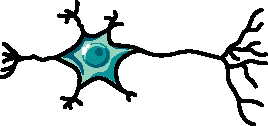
\includegraphics[width=\linewidth]{graphics/neuron}
    \caption[Schematic diagram of a neuron]{%
        Schematic diagram of a neuron.
        A typical neuron has a dendrites, a cell body, and a single axon; 
        the dendrites receive input signals from other neurons,
        and propagates output signals along the axon.
    }
    \label{fig:neuron}
\end{marginfigure}

\begin{marginfigure}%
	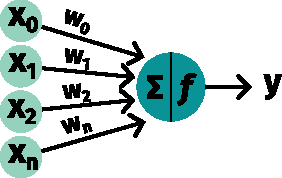
\includegraphics[width=\linewidth]{graphics/perceptron}
	\caption{Schematic diagram of a perceptron}
    \label{fig:perceptron}
\end{marginfigure}

%%%%%%%%%%%%%%%%%%%%%%%%%%%%%%%%%%%%%%%%%%%%%%%%%%%%%%%%%%%%%%%%%%%%%%%%%%%%%%%

Neural networks have been designed
using the archicteture of neurons in a human brain as inspiration.
The simplest model is that of a perceptron, 
which can be seen as a computational approximation
of a real neuron or nerve cell%
\autocite{charniakIntroduction2019}.
A typical neuron has many dendrites, a cell body, and a single axon 
(Figure~\ref{fig:neuron}).
The dendrites carries the input signal to a neuron,
and if the cumulative signal is great enough%
\sidenote{
    This threshold is known as 
    the \textit{threshold potential},
    and is typically between -50 and -55 mV.
}, 
then the neuron will propagate an action potential down the axon%
\autocite{seifterConcepts2005}.
In similar fashion, a perceptron receives may receive many different inputs
and produces a single output (Figure~\ref{fig:perceptron}).
In the case of a neuron, the \enquote{all-or-none} principle means
that nerve cells either signals at full strength or not all.
For a perceptron, this priniciple can be emulated
with the followingly step function:

\begin{equation}
    f_{\phi}(\mathbf{x})  = 
        \begin{cases}
            1 & \text{if } b + \mathbf{w} \cdot \mathbf{x} > 0\\
            0 & \text{otherwise}
        \end{cases}
\end{equation}

By combing many thousands of such neurons,
in a multilayer-perceptron or artificial neural network,
we can create a model that, 
can learn even the most complex of patterns.
Deep learning is at its core a form of representation learning.
Each layer in a neural network is a different representation,
and by stacking several of such layers on top of each others,
the representation in one hidden layer
feeds into the next layer and
is thereby being transformed into an even more abstract representation%
\autocite{estevaGuide2019}.

%%%%%%%%%%%%%%%%%%%%%%%%%%%%%%%%%%%%%%%%%%%%%%%%%%%%%%%%%%%%%%%%%%%%%%%%%%%%%%%
% insert example of abstract representations in a computervis model
%%%%%%%%%%%%%%%%%%%%%%%%%%%%%%%%%%%%%%%%%%%%%%%%%%%%%%%%%%%%%%%%%%%%%%%%%%%%%%%


\section{Regularization}

One approach to avoid overfitting in neural networks
is a technique known as dropout.
At each step of model training,
a random set of nodes in the network are disabled.
In a sense, the result is a rough approximation of 
an ensemble of different networks.


Dropout introduces noise during training
and thereby forces the network to be less senstive of noise.
Hidden units trained with dropout needs to be useful 
with or without the presence of neighboring units.

%%%%%%%%%%%%%%%%%%%%%%%%%%%%%%%%%%%%%%%%%%%%%%%%%%%%%%%%%%%%%%%%%%%%%%%%%%%%%%%

\section{Miscellaneous}

In his review on artificial intelligence in medicine%
\autocite{topolHighperformance2019}, 
Eric Topol expresses his view that in the future
\blockquote{%
almost every type of clinician, ranging from specialty doctor to paramedic,
will be using AI technology, and in particular deep learning [...]
}.

The ability to predict adverse outcomes could make  
healthcare resources more efficient.

Systematic deugging and continuous monitoring and validation 
is of utmost importance if we are to release AI algorithms into the wild%
\autocite{topolHighperformance2019}.

There has been much discussion about, and there are many opinions on, 
the black-box nature of many machine learning algorithms and 
how it should or should not affect the clinical use of such 
\autocite{topolHighperformance2019, gunningXAI2019, vanderveldenExplainable2022}.


In computer vision tasks in the medical domain,
deep-learning models have achieved physician-level performance
in many different diagnostic tasks
ranging from \todo{finish sentence}.
   
\chapter{Time-to-Event Prediction with Neural Networks}
\label{survival-analysis}

% marginnote {{{
\marginnote{%
    \setlength{\parindent}{0pt}
    \vskip 1em
    What is survival analysis?
    \begin{description}[leftmargin=!, labelwidth=3em]
        \item[outcome] time until an event occurs.
            Can be measured in seconds, days, months, etc.
        \item[event] death, relapse, remission, engine failure, etc.
    \end{description}
    
    \begin{center}
    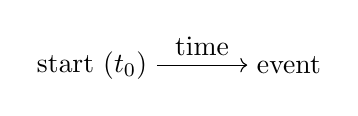
\begin{tikzpicture}
        \noindent
        \node (a) at (2.5, 0) {event};
        \node (b) at (0, 0) {start (\(t_0\))} edge ["time", ->] (a);
    \end{tikzpicture}
    \end{center}
}
% }}}

In the previous chapter, 
I gave an overview of machine learning and neural networks,
highlighting key ideas and concepts related to the studies in this thesis.
Neural networks specifically, 
were used in \studyii{} and \studyiii{} to develop
prediction models for ischemic heart disease.
These models, however, diverge from classical neural network methods.
Instead, they include modifications that make them applicable
in modelling and analysis of time-to-event data.
This chapter will provide an introduction to the fundamentals
of survival analysis and will cover the
theory that enables the implementation of such analyses with
neural network models.
% The chapter concludes with a discussion on different 
% validation methods for time-to-event prediction models.

\section{What is Survival Analysis?}

Generally, 
survival analysis is the collection of statistical methods
for the modelling and analysis of time-to-event data,
which is data where the outcome variable of interest 
is the time until \enquote{something} happens.~%
~\autocite{kleinbaumSurvival2011}
This \enquote{something} is a particular event of interest,
which, depending on the type of analytical problem, 
could be cancer relapse, 
diabetes remission,
or death.
In cardiovascular research, 
common examples of time-to-event outcomes include
\begin{enumerate*}
    \item time to death due to any cause (all-cause mortality)
    \item time to death due to a specific cause,
        e.g. sudden cardiac arrest
    \item time to first occurence of a \ac{MACE}
\end{enumerate*}.
To figure out what processes and characteristics 
that are associated with such events, 
in survival analysis, we try to model the relationship between
explanatory variables and the number of weeks, months, or years 
until that particular event is likely to occur. 

% marginnote{{{
\marginnote{%
    Survival analysis have applications outside biomedical research.
    In engineering, it is called \textit{reliability analysis} and
    is used to model the time-to-failure of system-critical components 
    such as e.g. bearings or valves.
}% }}}

Although this task can be daunting in its own right, 
an additional complication to survival analysis 
is the presence of observations that are subject to 
censoring.
This concept, censoring, refers to cases 
where the event of interest has not been observed 
before the end of follow-up, 
e.g. when a study or experiment has to be stopped.
In such cases, 
we would know that a given subject did not experience a relapse 
in the three months he or she was included in the study, 
but after the study period ends, 
we have no information on the status of the patient. 
Including and utilizing this partial information
is a cornerstone in many survival analysis problems.

There exists different forms of censoring,
such as right censoring, left censoring, and interval censoring.
In the study designs used throughout this thesis 
we have only had to deal with right censoring,
the most common form of censoring,
so the two other types will not be described further.
See instead the text book by \citeauthor{kleinSurvival2003} 
for more details on this.
~\autocite{kleinSurvival2003}

\section{Fundamentals of Survival Analysis}

In survival analysis, 
the central outcome variable is survival time,
a non-negative random variable denoted as \(T\). 
When refering to specific values of \(T\), 
a lower case \(t\) is typically used.  
A survival dataset \(\mathfrak{D}\) of size \(N\) is given by
\begin{equation}
    \mathfrak{D}_N = \{(t_i, \sigma_i, \vec{x}_i) \mid i = 1, \ldots, N\} 
\end{equation}
where \(t_i = \min(T_{i}, C_i) \) is the survival time 
for the \(i\)th subject,
with \(T_i\) denoting the survival time
and \(C_i\) denoting the censoring time. 
Also, \(\vec{x}_i = (x_1, x_2, \dots, x_p)'\) is the covariate vector
and \(\sigma_i\) is the event indicator, which is defined as
\begin{equation}
    \label{eq:sigma-def}
    \sigma_i =
        \begin{cases}
            0 & \text{if subject is censored} \; (T_i >    C_i) \\
            1 & \text{if event is observed} \; (T_i \leq C_i)
        \end{cases}
\end{equation}

In the following, I will initially be assuming that \(T\) is 
continuous and that there is an absence of competing risks, 
however both of these assumptions will later be relaxed in the discussion 
of competing risks and discrete-time survival analysis.

\subsection{Basic Survival Quantities}
\label{sub:survival-quantities}

% figure: theoretical survival function{{{
\begin{marginfigure}%
	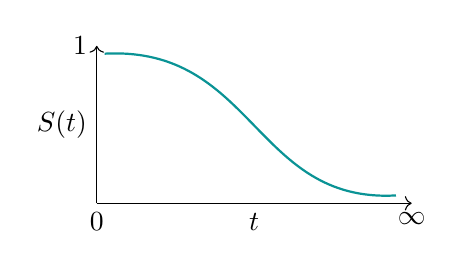
\begin{tikzpicture}[scale=2]
	  \draw[->] (0, 0) --  (2,0) 
		node[pos=0.0, below] {$0$}
		node[pos=0.5, below] {$t$}
		node[pos=1.0, below] {$\infty$};
	  \draw[->] (0, 0) --  (0,1) 
		node[pos=1.0, left] {$1$}
		node[pos=0.5, left] {$S(t)$};
	  \draw[-, color=color2, thick] 
		(0.05, 0.95) .. controls (1, 1) and (1, 0) .. (1.90, 0.05);
	\end{tikzpicture}
    \caption[A Theoretical Survival Function]}}

In survival analysis, 
the central function of interest is 
the survival function \(S(t)\), 
that represents the probability 
of an individual still being alive after 
some specified duration of time, we have that 
%
\begin{equation}
    S(t) = \PR (T > t), \quad 0 < t < \infty.
\end{equation}

The survival function is 
the integral of the probability density function, \(f(t)\),
and is the complement to the cumulative distribution function, \(F(t)\),
which means that
~\autocite{kleinSurvival2003}
%
\begin{equation}
    S(t) = 1 - F(t) 
    \quad \text{and} \quad 
    S(t) = \int_{t}^{\infty} f(u) \, \diff u
\end{equation}

Another fundamental quantity is the hazard function, or hazard rate,
which represents the instantaneous failure rate at a given timepoint,
and is defined as
%
\begin{equation}
    \label{eq:hazard-function}
    \lambda(t) = \lim_{\Delta t \to 0} 
        \frac{\PR (t \leq T < t + \Delta t \mid T \geq t)}{\Delta t}
\end{equation}
% 
from which it can be shown that
~\autocite{kleinSurvival2003}
%
\begin{equation}
    \lambda(t) = \frac{f(t)}{S(t)} = -\frac{\diff}{\diff t} \ln[S(t)].
\end{equation}
%
and thus the hazard function completely describes the distribution of \(T\),
such that all the the other quantities can be obtained from it---%
as well as the other way around.

In terms of its interpretation, 
from \cref{eq:hazard-function} it follows that \(\lambda(t)\Delta t\) 
is a measure of the conditional probability of failure in a small time
window, given that the individual is still alive at time \(t\).
~\autocite{kleinSurvival2003}

Analogous to the relation between \(f(t)\) and \(F(t)\), 
integrating \(\lambda(t)\) with resport to \(t\),
we obtain cumulative hazard function, defined as
%
\begin{equation}
    \Lambda(t) = \int_{0}^{t} \lambda(u) \, \diff u = -\ln[S(t)].
\end{equation}

\subsection{The Kaplan-Meier Estimator}

The survival function of a population,
can be estimated using the Kaplan-Meier method,
which is the standard estimator of the survival function.
~\autocite{kaplan1958nonparametric}
~\autocite{kleinSurvival2003}
In this approach, 
the distinct failure times are ordered such that%
\footnotemark
\begin{equation*}
    t_{(1)} < t_{(2)} < \ldots < t_{(j)},
\end{equation*}
%
and we introduce two quantities to keep track of
the number of failures \(\widebar{D}(j)\), 
as well as the number of subjects still at risk \(\widebar{A}(j)\).
They are defined as
\begin{equation}
\begin{aligned}
    \bar{D}(j) &= \card \{i \in \{1, \dots, n\} \mid t_i = t_{(j)}, \sigma_i = 1\} \\
    \bar{A}(j) &= \card \{i \in \{1, \dots, n\} \mid t_i > t_{(j)}\},
\end{aligned}
\end{equation}
and the Kaplan-Meier estimator can then be formulated as 
\begin{equation}
    \widehat{S}(t)
    =   \prod_{j \mid t_{(j)} \leq t} 
        \frac{
            \bar{A}(j) -
            \bar{D}(j)
        }{
            \bar{A}(j)
        }
    =   \prod_{j \mid t_{(j)} \leq t} 
        1 - \frac{
            \bar{D}(j)
        }{
            \bar{A}(j)
        }.
\end{equation}

\footnotetext{%
    Following the example of [\cite{kleinbaumSurvival2011}], 
    the \(t\)'s denoted with subscripts within parentheses \(t_{(j)}\)
    refers to the \(j\)th element of the ordered distinct failure times and
    are thus different from \(t_1, t_2, \ldots, t_i\) that refers to the 
    observed failure time of subject \(1\), \(2\), and \(i\)
}

The Kaplan-Meier estimator is thus as step-function that decreases
after each observed event.
While the Kaplan-Meier estimator is useful 
for summarising the survival of a population, 
it does not account for the effect of covariates.
Instead, another approach is needed for regression analyses.

\subsection{Cox's Proportional Hazards Model}

To describe and model the relationship between explanatory variables
and time-to-event phenomenons, a widely used statistical model is 
the Cox proportional hazards model. 
~\autocite{coxRegression1972}
This model seeks to model the hazard function over time \(t\),
of an individual with a covariate vector \(\vec{x} = (x_1, x_2, \dots)'\),
and assumes that it takes the form of
%
\begin{equation}
    \label{eq:cox}
    \widehat{\lambda} (t \,|\, \vec{x}) = \hzt \exp [g(\vec{x})],
\end{equation}
%
where \(\hzt\)
is an unspecified baseline hazard function,
and \(g(\vec{x})\) is some parametric function.
For this reason, the Cox model 
is referred to as a semi-parametric model.
In its classical formulation, 
this function is a linear combination of parameters 
\(\vec{\beta}\) and covariates \(\vec{x}\),
as given by

\begin{equation}
    g(\vec{x}) 
    = \vec{\beta}' \vec{x} 
    = \beta_1 x_1 + \beta_2 x_2 + \ldots + \beta_p x_p
\end{equation}

In estimation of the parameters \(\vec{\beta}\),
the baseline hazard \(\hzt\) is treated as a nuisance function
and the coefficients are estimated by
maximising a partial likelihood
in which \(\hzt\) has been abstracted away.
~\autocite{kalbfleischStatistical2002}

A central assumption in the Cox model, 
at least in the standard version with fixed covariates
(\(\vec{\beta}\) instead of \(\vec{\beta}(t)\)),
is that of proportional hazards.
Let \(\vec{x}\) and \(\vec{x}'\) be two different 
covariate vectors, now the ratio between their
respective Cox-estimated hazards is

\begin{equation}
    \label{eq:hazard-ratio}
    \begin{aligned}
    \frac%
        {\widehat{\lambda}(t \,|\, \vec{x} \hfill)}%
        {\widehat{\lambda}(t \,|\, \vec{x'})}
    &=
    \frac%
        {\hzt \exp (\vec{\beta}\cdot\vec{x}\hfill)}%
        {\hzt \exp (\vec{\beta}\cdot\vec{x'})} \\
    &=
    \frac%
        {\exp (\vec{\beta}\cdot\vec{x}\hfill)}%
        {\exp (\vec{\beta}\cdot\vec{x'})} \\
    &= \exp (\vec{\beta} \cdot (\vec{x} - \vec{x'}))
    \end{aligned}
\end{equation}

Since the right-hand side of the equation does not include a term for \(t\),
the hazard ratio between the two samples are constant and 
they are thus proportional to one another., 
This shows that by assuming the hazard takes the form of \cref{eq:cox},
then it is also assumed that the hazards between two subjects are proportional.
Although this assumption is a strong one, 
and the validity of the Cox model relies on it, 
the assumption makes interpretation of parameters easier.
~\autocite{tutzModeling2016}
For example, 
in an randomized clinical trial
studying the survival effect of a new type of medication, 
we can let \(x = 1\) represent the experimental treatment  
and \(x' = 0\) represent standard of care, 
then the hazard ratio in \cref{eq:hazard-ratio} takes the form of
%
\begin{equation}
      \exp \left(\beta (x - x')\right)
    = \exp \left(\beta (1 - 0)\right)
    = \exp (\beta ),
\end{equation}
%
which means that if \(\beta < 0\), 
then the hazard of the experimental treatment is 
\(\exp({\beta})\) times lower than standard of care
and should therefore be preferred.%
\sidenote{% 
This example is a slightly modified version of the 
one given in \cite[pp. 50]{tutzModeling2016}}


\section{Analysis of Competing Risks}

\begin{marginfigure}[3em]% {{{
    \tikzstyle{outcome}=[%
        rectangle, rounded corners, minimum height=5mm, fill=color3
    ]
    \centering
    \begin{tikzpicture}[x=0.60\linewidth, y=1cm]
    \graph [edge quotes={font=\scriptsize, fill=white}, 
            nodes      ={draw, outcome, sloped, minimum width=1cm}]{
        alive [fill=color4] -> dead [> "\(\lambda(t)\)" ];
    };
    \end{tikzpicture}
    \caption[A Single State Model]{
        A simple survival analysis setup 
        involves modelling a single transition between states 
        \enquote{alive} and \enquote{dead}.
    }
    \label{fig:ssm}
\end{marginfigure}% }}}

Up to this point, the description of concepts in survival analysis has
assumed the presence of only a single event type, such as all-cause mortality
(\cref{fig:ssm}).
In practice, particularly in clinical settings, 
this single-event model can be too restrictive,
and instead one needs to consider competing risks
(\cref{fig:msm}).
By definition, a competing risk is a secondary event whose occurence 
prevents the primary event from occuring.
For example,
in a study where the primary outcome is cardiovascular mortality,
deaths from non-cardiovascular causes are a competing risk.

In the following, 
we let \(R \in \{1, \dots, \kappa\}\) denote the \(\kappa\) different competing risks,
and then slightly update the definition of the event indicator \(\sigma_i\)
(\cref{eq:sigma-def}), such that
\begin{equation}
    \label{eq:sigma-def-2}
    \sigma_i =
        \begin{cases}
            0 & \text{if subject is censored} \; (T_i >    C_i) \\
            r & \text{if cause r is observed} \; (T_i \leq C_i, R = r).
        \end{cases}
\end{equation}

\begin{marginfigure}% {{{
    \tikzstyle{outcome}=[%
        rectangle, rounded corners, minimum height=5mm, fill=color3
    ]
    \centering
    \begin{tikzpicture}[x=0.60\linewidth, y=0.85cm]
    \graph [edge quotes={font=\scriptsize, fill=white}, 
            nodes      ={draw, outcome, sloped, minimum width=1cm}]{
        alive [fill=color4] -> {
            cause 1 [> "\(\lambda_1(t)\)" ],
            cause 2 [> "\(\lambda_2(t)\)" ],
            cause k [> "\(\lambda_\kappa(t)\)" ],
        };
    };
    \end{tikzpicture}
    \caption[A Multi-State Model]{
        A survival analysis setup with competing risks
        involves modelling transitions between states 
        \enquote{alive} and \(k\) different absorbing
        states, \enquote{cause 1} to \enquote{cause \(\kappa\)}
    }
    \label{fig:msm}
\end{marginfigure}
% }}}

\subsection{Cause-Specific Survival Quantities}

To describe time-to-event phenomena with competing risks, 
we introduce the cause-specific hazard function and 
cumulative-incidence function.
With \(R \in \{1, \dots, \kappa\}\) denoting the \(\kappa\) different competing risks, 
the cause-specific hazard function is defined as
\begin{equation}
    \lambda_r(t) = \lim_{\Delta t \to 0} 
        \frac{\PR (t \leq T < t + \Delta t, R=r \mid T \geq t)}{\Delta t}
\end{equation}
where \(r\) refers to a specific value of \(R\).
The cause-specific cumulative incidence function is defined as
~\autocite{kalbfleischStatistical2002}
\begin{equation}
    F_r(t) = \PR(T \leq t, R = r).
\end{equation}

The overall hazard and cumulative incidence, 
which combines failures of any of the \(\kappa\) causes,
correspond to the hazard function 
and the cumulative distribution function 
in the single-event setting, that is
\begin{equation}
    \lambda(t) = \sum_{r=1}^{\kappa} \lambda_r(t)
    \quad \text{and} \quad
    F(t) = \sum_{r=1}^{\kappa} F_r(t).
\end{equation}

\subsection{The Aalen-Johansen Estimator}

In the competing risk setting, 
some of the methodology previously presented
have to be slightly adjusted.
For example, 
simply treating competing events as censored 
and applying the standard Kaplan-Meier estimator, 
would lead to a biased estimate of \(F(t)\).
~\autocite{pepeKaplan1993}
Instead, an alternative approach is the Aalen-Johansen estimator
that allows estimation of the cause-specific cumulative incidence.
~\autocite{aalenEmpirical1978}
Of note, the Aalen-Johansen is a general method for estimating
transition probabilities in state-transition models,
and can be used to describe complex multi-state models,
including those with repeated events and with non-terminal states.
~\autocite{survival-package}
However, we will be assuming a standard competing-risk setting
with \(\kappa\) different terminal states, 
as depicted in \cref{fig:msm}.
 
If we again order the distinct failure times, 
corresponding to any cause, 
such that
\(t_{(1)} < t_{(2)} < \ldots < t_{(j)}\),
and update the definition of \(\bar{D}(j)\) to keep track of cause-specific
events, such that we have
\begin{equation}
\begin{aligned}
    \bar{D}(j, r) &= \card \{i \in \{1, \dots, n\} \mid t_i = t_{(j)}, r_i = r\} \\
    \bar{A}(j)    &= \card \{i \in \{1, \dots, n\} \mid t_i > t_{(j)}\}.
\end{aligned}
\end{equation}
Now, the Aalen-Johansen estimator of the cumulative incidence function
can be defined as 

\begin{equation}
    \widehat{F}_r(t)
    =   \sum_{j \mid t_{(j)} \leq t}{
        \!\!
        \widehat{S}(t_{(j-1)})
        \frac{\bar{D}(j, r)}{\bar{A}(j)}
    }
\end{equation}

\section{Time-to-Event Prediction}

Up until now, 
I have outlined various concepts foundational to survival analysis,
focusing primarily on quantities and statistics of time-to-event outcomes
at a popoulation level.
These measures play an important role in understanding 
and interpretation of survival data.

In the context of precision medicine, however,
the emphasis shifts towards making individualized predictions
taking distinct patient-level characteristics into account.
Consequently, as described in \cref{chap:ml-and-nn}, 
the primary concern lies in 
making accurate predictions on unseen data,
rather than in the exploration of disease etiology and underlying mechanisms.

For prediction of time-to-event outcomes, classical approaches 
include models based on the previously presented semi-parametric Cox model 
as well as various parametric survival models, 
such as those based on exponential, Weibull, or log-normal distributions.
~\autocite{kleinSurvival2003}
This thesis, however, 
explores the use of contemporary machine learning methods 
in time-to-event prediction,
with a particular emphasis on the application of neural networks.

\subsection{Neural Networks and Time-to-Event Outcomes}

The first application of neural networks for time-to-event prediction
was demonstrated by
\citeauthor{faraggiNeural1995} in
\citeyear{faraggiNeural1995},
and involves parameterising the parametric part of the Cox model
with a neural network, 
such that the \(g(\vec{x})\) term in \cref{eq:cox} is a 
flexible neural network model instead of a simple linear function.
\autocite{faraggiNeural1995}

\vspace{.5em}
\begin{equation*}
    \widehat{\lambda} (t \,|\, \vec{x}) = \hzt \exp [
    \eqnmarkbox[color2]{node1}{
        g(\vec{x})
    }]
\end{equation*}
\annotate[yshift=.6em]{left}{node1}{use neural network}

This approach was later further refined
in the \emph{DeepSurv} paper from 
\citeyear{katzmanDeepSurv2018a},
in which modern neural network techniques
were added to Faraggi-Simon framework, 
which markedly improved its usefulness.
~\autocite{katzmanDeepSurv2018a}
\citeauthor{katzmanDeepSurv2018a} showed that the flexibility 
offered by neural networks led to increased performance
in both synthetic and real-life time-to-event prediction applications
compared to a standard Cox model.
However, the \emph{DeepSurv} approach is still limited by the 
assumption of proportional hazards.

\subsection{Overview of Approaches}

Recently, there have been considerable interest in neural network-based
time-to-event prediction models, and as a consequence, many new methods 
have since been developed.
For a thorough overview of the existing approaches, 
\textcite{wiegrebeDeep2023} and 
\textcite{kvammeContinuous2021} provide valuable insights.
Generally, two prevailing types of approaches exists:
continuous-time methods based on the Cox model, 
which includes \emph{DeepSurv},
and discrete-time methods as exemplified by 
\textcite{leeDeepHit2018} and \textcite{gensheimerScalable2019}.

The discrete-time approaches offer several advantages that 
make them particularly relevant for neural network. 
Furthermore, they have been shown to offer better predictive
performance compared to the Cox-based methods.
~\autocite{kvammeContinuous2021, leeDeepHit2018, gensheimerScalable2019}
Notably, \emph{DeepHit}\autocite{leeDeepHit2018}
and \emph{Logistic-Hazard}\autocite{gensheimerScalable2019}
are the two most cited papers in this context as of the time of writing.
Among these and other tested approaches,
\textcite{kvammeContinuous2021} found that 
DeepHit offers excellent discrimination but suffers from poor calibration.
In contrast, the Logistic-Hazard model have nearly as good discrimination
and also significantly better calibration. 
Consequently, the Logistic-Hazard model, and an extension hereof, 
was chosen for application in 
\studyii{} and \studyiii{}.

In the following section, I will be giving a brief description of
this discrete-time formulation of time-to-event analysis and 
elaborate on the Logistic-Hazard model in more detail.

\section{Discrete-Time Survival Analysis}

Most textbooks on survival analysis treats survival time as continuous, 
and that is also usually the case across the biomedical litterature.
However, handling time as a something discrete can be advantegous.
In practice, most measurements of time is inherently discrete 
with durations being recorded in, for example, days; months; and weeks.
The continuous time approaches presented earlier in this chapter, 
are also applicable to discrete time data,
however, methods designed specifically for discrete time-to-event 
data have some advantages~\autocite{tutzModeling2016}:

\begin{itemize}
    \item If observed event times are inherently discrete, 
        then modelling them as such is arguably more appropriate. 
    \item In the discrete-time setting, hazards can be formulated as 
        conditional probabilities which are much more intuitive to 
        both interpret and understand.
    \item Discrete time-to-event models are more easily transferred to 
        other more general purpose modelling frameworks 
        such as generalized linear models, random survival forests, 
        neural networks.
\end{itemize}

The latter point is the main motivation behind both 
the \emph{DeepHit} and \emph{Logistic-Hazard} approach.
For a complete overview of the theory enabling these two approaches,
the book by \textcite{tutzModeling2016} is a valuable resource, 
and serves as the main source of reference for the following.

\subsection{Notation and Definitions}

In the discrete-time framework, 
continuous follow-up time \(\Tic\) is divided into \(q\) contiguous intervals,
that is
%
\begin{equation*}
	(0, a_1], (a_1, a_2], \dots, (a_{q-1}, a_q]
\end{equation*}
%
and \(\Tid \in \{1, \dots, q\}\) is a discrete random  variable
such that if \(\Tid = \tid\) is observed, then the event 
falls in the interval \((a_{\tid-1}, a_{\tid}]\).
Similarly, the discretized censoring time is \(\Cid \in \{1, \dots, q\}\).

With this discrete time scale, 
the distribution of \(\Tid\), 
given some vector of covariates \(\vec{x}\),
can be described using discrete equivalents of the previously 
outlined basic quantities of survival analysis, that is
%
\begin{align}
    \text{probability mass function:} \qquad
    f(\tid \giv \vec{x}) 
    &= \PR (\Tid = \tid \mid \vec{x}) \\
    %
    \text{cumulative mass function:} \qquad
    F(\tid \giv \vec{x}) 
    &= \PR (\Tid \leq \tid \mid \vec{x}) \\
    %
    \label{eq:discrete-hazard}
    \text{hazard function:} \qquad
    \lambda(\tid \giv \vec{x}) 
    &= \PR (\Tid = \tid \mid \Tid \geq \tid, \vec{x}) \\
    %
    \text{survival function:} \qquad
    S(\tid \giv \vec{x}) 
    &= \PR (\Tid > \tid \mid \vec{x})
\end{align}

\subsection{The Logistic-Hazard Model}

\Citeauthor{gensheimerScalable2019}'s approach, 
which they refer to as \enquote{Nnet-survival},
~\autocite{gensheimerScalable2019}
is more accurately characterized as the Logistic-Hazard method, 
as described in \textcite{kvammeContinuous2021}.
In the Logistic-Hazard method, 
the time-to-event data is described by 
modelling the effect of covariates on the discrete hazard function 
(\cref{eq:discrete-hazard}) 
using a neural network.
The concept is not novel, 
employing the discrete hazard for statistical modeling is a common method, 
as covered extensively in \textcite{tutzModeling2016}. 
In addition, a neural-network based model with the same general idea 
was presented by \citeauthor{brownUse1997} in 1997.
~\autocite{brownUse1997}
However, 
\citeauthor{gensheimerScalable2019} were the first to adapt the approach
to current neural network methodologies.

\subsection{Log-Likelihood of the Discrete Hazard}

Let \(\mathfrak{D}_{\mathrm{d}}\) 
be a discrete-time survival dataset of size \(N\),
\begin{equation}
    \mathfrak{D}_{\mathrm{d}} = 
    \{(\tid_i, \sigma_i, \vec{x}_i) \mid i = 1, \ldots, N\},
\end{equation}
where \(\tid_i\) is the discretized survival time, 
\(\sigma_i\) is the event indicator as defined in \cref{eq:sigma-def},
and \(\vec{x}_i = (x_1, x_2, \dots, x_p)'\) is the feature vector.
With the assumption of \emph{noninformative censoring},
~\autocite{kalbfleischStatistical2002}
in the Logistic-Hazard model, 
the contribution of the \(i\)th individual to the likelihood function
can be shown to be  
~\autocite{tutzModeling2016}
\begin{equation}
    \Lik_i = %
    \begin{cases}
        \PR (\Tid_i = \tid_i) & \text{if non-censored} \\
        \PR (\Tid_i > \tid_i) & \text{if censored}.
    \end{cases}
\end{equation}

These two probabilities can be expressed using the discrete hazards,
as it can be seen that
\begin{align}
    \begin{split}
    \PR (\Tid = \tid) 
    &= \PR (\Tid = \tid \mid \Tid \geq \tid) \PR (\Tid  \geq \tid) \\
    &= \PR (\Tid = \tid \mid \Tid \geq \tid) \PR (\Tid  > \tid - 1) \\
    &= \lambda (\tid) \, \prod_{s=1}^{\tid - 1} (1 - \lambda(s))
    \end{split} \\
    \intertext{and similarly}
    \begin{split}
    \PR (\Tid > \tid) 
        &= \PR (\Tid > \tid \mid \Tid \geq \tid) \PR (\Tid  \geq \tid) \\
        &= (1 - \PR (\Tid = \tid \mid \Tid \geq \tid)) \PR (\Tid  \geq \tid) \\
        &= (1 - \PR (\Tid = \tid \mid \Tid \geq \tid)) \PR (\Tid  > \tid - 1) \\
        &= \prod_{s=1}^{\tid} (1 - \lambda(i)).
    \end{split}
\end{align}

Now, by introducing an indicator function, 
defined according to \textcite{tutzModeling2016} as 
\begin{equation}
    \label{eq:lh-indicator}
    \bar{y}_i(\tid) = \begin{cases}
        1, & \text{if individual fails in \((a_{\tid-1}, a_{\tid}]\),} \\
        0, & \text{if individual survives \((a_{\tid-1}, a_{\tid}]\),}
    \end{cases}
\end{equation}
and by including the discrete hazard function and the covariates, 
the likelihood contribution for the \(i\)th individual can be expressed as
\begin{equation}
    \label{eq:lh-likelihood}
    \Lik_i = \prod_{s=1}^{\tid_i} 
        \lambda(s \giv \vec{x}_i)^{\bar{y}_i(s)}
        (1 - \lambda(s \giv \vec{x}_i))^{1 - \bar{y}_i(s)}.
\end{equation}

The total log-likelihood of all datapoints then gives the loss-function
used in the Logistic-Hazard model, 
~\autocite{gensheimerScalable2019, tutzModeling2016}
which can be expressed
\begin{equation}
    \label{eq:lh-loglikelihood}
    \lik = 
        \sum_{i = 1}^{N} 
            \sum_{s=1}^{\tid_i} 
                \bar{y}_i(s) \log (\lambda(s\giv\vec{x}_i))
                + (1 - \bar{y}_i(s)) \log (1 - \lambda(s\giv\vec{x}_i)).
\end{equation}

\subsection{Loss Function Explained}

\def\y#1#2{\hat{\lambda}_{#1#2}}
\def\yy#1#2{1\!-\!\y{#1}{#2}}

As an example, the following set of observations with discretized 
time-to-event data with a single risk, e.g. all-cause mortality, 
and a follow-up time that have been discretized into seven contiguous intervals,
constitutes a survival dataset.

\begin{equation}
\begin{tabular}{r  ccccc}
    \toprule
    subject   \(i\)      & 1 & 2 & 3 & 4 & 5 \\
    \midrule
    time    \(\tau_i\)   & 5 & 7 & 4 & 5 & 3 \\
    event   \(\sigma_i\) & 1 & 1 & 0 & 0 & 1 \\
    \bottomrule
\end{tabular}
\end{equation}

In this setting,  using the Logistic-Hazard model, 
the neural network output for this dataset is a 2-dimensional
matrix with \(5\) rows  (subjects) and \(7\) columns (time intervals),
and each entry is the predicted conditional hazard for the
specific subject at a specific timepoint. We can write this as
\begin{equation}
\hat{\bm{\Lambda}}= \!\!\!\!
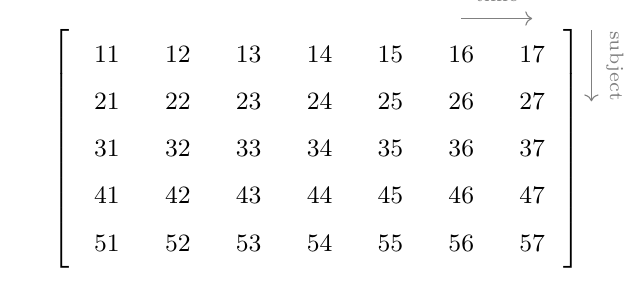
\begin{tikzpicture}
[   on grid,
    font = \small,
    baseline = -.7ex,
    inner sep=1pt,
    outer sep=0pt,
    minimum width=9mm,
    minimum height=6mm,
    every left delimiter/.style={xshift=2.5ex},
    every right delimiter/.style={xshift=-3.0ex}
]
\matrix (pred) [
	matrix of math nodes, 
    left delimiter={[}, 
    right delimiter={]},
]{ 
\y{1}{1} & \y{1}{2} & \y{1}{3} & \y{1}{4} & \y{1}{5} & \y{1}{6} & \y{1}{7} \\
\y{2}{1} & \y{2}{2} & \y{2}{3} & \y{2}{4} & \y{2}{5} & \y{2}{6} & \y{2}{7} \\
\y{3}{1} & \y{3}{2} & \y{3}{3} & \y{3}{4} & \y{3}{5} & \y{3}{6} & \y{3}{7} \\
\y{4}{1} & \y{4}{2} & \y{4}{3} & \y{4}{4} & \y{4}{5} & \y{4}{6} & \y{4}{7} \\
\y{5}{1} & \y{5}{2} & \y{5}{3} & \y{5}{4} & \y{5}{5} & \y{5}{6} & \y{5}{7} \\
};
\useasboundingbox[anchor=center] (pred.north west) rectangle (pred.south east);
\draw[->, black!50] ([xshift=2ex] pred-1-7.north east) -- ([xshift=2ex] pred-2-7.east)
    node [midway, font=\scriptsize, above, sloped] {subject};
\draw[->, black!50] ([yshift=1ex] pred-1-6.north) -- ([yshift=1ex] pred-1-7.north)
    node [midway, font=\scriptsize, above] {time};
\end{tikzpicture}
\end{equation}

Now, the indicator function can be computed 
using the defintion in \cref{eq:lh-indicator}
and the observed data \(\tid_i\) and \(\sigma_i\). 
In matrix form, the output of this function is
\begin{equation}
\bar{\bm{Y}}= \!\!\!\!
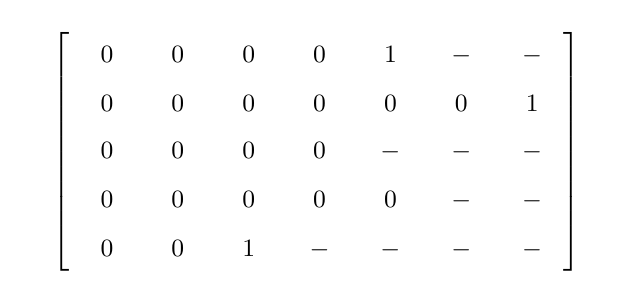
\begin{tikzpicture}
[   on grid,
    font = \small,
    baseline = -.7ex,
    inner sep=1pt,
    outer sep=0pt,
    minimum width=9mm,
    minimum height=6mm,
    every left delimiter/.style={xshift=2.5ex},
    every right delimiter/.style={xshift=-3.0ex}
]

\matrix (mask) [
	matrix of math nodes, 
    left delimiter={[}, 
    right delimiter={]}
]{ 
0 & 0 & 0 & 0 & 1 & - & - \\
0 & 0 & 0 & 0 & 0 & 0 & 1 \\
0 & 0 & 0 & 0 & - & - & - \\
0 & 0 & 0 & 0 & 0 & - & - \\
0 & 0 & 1 & - & - & - & - \\
};
\useasboundingbox[anchor=center] (mask.north west) rectangle (mask.south east);
\end{tikzpicture}
\end{equation}

Now, combining these two matrices according to the formula
in \cref{eq:lh-likelihood}, we obtain the likelihood in matrix form as
\begin{equation}
    \mathcal{L}(\bm{\hat{\Lambda}}, \bm{\bar{Y}}) = \!\!\!\!
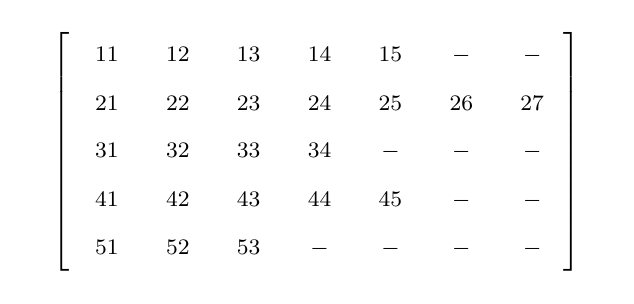
\begin{tikzpicture}
[   on grid,
    font = \small,
    baseline = -.7ex,
    inner sep=1pt,
    outer sep=0pt,
    minimum width=9mm,
    minimum height=6mm,
    every left delimiter/.style={xshift=2.5ex},
    every right delimiter/.style={xshift=-3.0ex}
]
\matrix (loss) [
	matrix of math nodes, 
    left delimiter={[}, 
    right delimiter={]},
    nodes={font=\footnotesize}
]{ 
\yy{1}{1} & \yy{1}{2} & \yy{1}{3} & \yy{1}{4} & \y{1}{5}  & -         & -         \\
\yy{2}{1} & \yy{2}{2} & \yy{2}{3} & \yy{2}{4} & \yy{2}{5} & \yy{2}{6} &  \y{2}{7} \\
\yy{3}{1} & \yy{3}{2} & \yy{3}{3} & \yy{3}{4} & -         & -         & -         \\
\yy{4}{1} & \yy{4}{2} & \yy{4}{3} & \yy{4}{4} & \yy{4}{5} & -         & -         \\
\yy{5}{1} & \yy{5}{2} & \y{5}{3}  & -         & -         & -         & -         \\
};
\useasboundingbox[anchor=center] (loss.north west) rectangle (loss.south east);
\end{tikzpicture}
\end{equation}
from which the log-likelihood, \cref{eq:lh-loglikelihood}, is then
\begin{equation*}
    \small
\begin{split}
    \mathscr{l}(\bm{\hat{\Lambda}}, \bm{\bar{Y}})
    &={} \log (\yy{1}{1}) + \log(\yy{1}{2}) + \log(\yy{1}{3}) + \log(\yy{1}{4}) 
     +  \log(\y{1}{5}) \\ 
    &+{} \log (\yy{2}{1}) + \log(\yy{2}{2}) + \log(\yy{2}{3}) + \log(\yy{2}{4}) 
     +  \log(\yy{2}{5}) + \log(\yy{2}{6}) +  \log(\y{2}{7}) \\
    &+{} \log (\yy{3}{1}) + \log(\yy{3}{2}) + \log(\yy{3}{3}) + \log(\yy{3}{4}) \\
    &+{} \log (\yy{4}{1}) + \log(\yy{4}{2}) + \log(\yy{4}{3}) + \log(\yy{4}{4}) 
    + \log(\yy{4}{5})  \\
    &+{} \log (\yy{5}{1}) + \log(\yy{5}{2}) + \log(\y{5}{3} )
\end{split}
\end{equation*}
  
\chapter{Overview of Data Resources}
    

\part{Outline of Studies}
\chapter{Study I: Comorbidity Clustering in Ischemic Heart Disease}
\label{chap:study1-outline}

In this chapter, I provide a summary of the work from \studyi{}.
I describe the background and rationale,
outline essential methodological details,
and discuss the main research findings.

The manuscript, titled \enquote{%
Subgrouping multimorbid patients with ischemic heart disease by
means of unsupervised clustering: A cohort study of 72,249
patients defined comprehensively by diagnoses prior to
presentation}, is currently under revision.
An earlier version have been deposited on the medRxiv preprint server. 
\autocite{haueSubgrouping2023}
The revised, full-length manuscript is included in 
\cref{chap:study1-paper}.

\section{Background and Rationale}

\Ac{IHD} is highly heterogeneous in its onset, burden, and progression.
As delineated in \cref{chap:precision-medicine}, its manifestations range from 
\ac{AMI} to slowly progressing chronic coronary syndromes.
This heterogeneity is partly explained, and further complicated,
by the fact that most patients with \ac{IHD} have one or more 
comorbidities.
Current clinical practice is historically mainly based on a single-disease paradigm
and thus, complexities imposed by concurrent comorbid diseases are therefore 
often overlooked.
~\autocite{formanMultimorbidity2018}

In this study, we sought to characterise the spectrum of multimorbidity
in \ac{IHD}. 
We adopted a data-driven strategy, using unsupervised machine learning
methods to identify and characterize subgroups 
with distinct comorbidity patterns. 
Our hypothesis centered on the notion that the 
variety and types of comorbidities,
here classified according to \acsu{ICD-10} codes, 
could facilitate the identification of distinct and clinically relevant 
patient clusters in \ac{IHD}.

\section{Study Design and Outcomes}

We linked the \ac{BTH} dataset to the \ac{LPR} and \ac{DAR}, 
and identified all patients with an \ac{ICD-10} code for \ac{IHD},
who underwent \ac{CAG} or \ac{CCTA} between 2004 and 2016 
(\num{72249} patients in total).
We used the date of the first \ac{CAG} or \ac{CCTA} as the index date. 
All \ac{ICD-10} codes before this date were collected
for clustering analysis, excluding any \ac{IHD} codes (\ac{ICD-10}: I20-25).

In our study, we defined two main outcomes to assess the risk
profiles of the different multimorbidity subgroups: (i) new ischemic events
and (ii) mortality from non-\ac{IHD} causes.
New ischemic events, a composite outcome, included 
(a) hospital admission for \ac{AMI} or \ac{UA} after 30 days of follow-up
(b) revascularization procedures unrelated to the index \ac{CAG}/\ac{CCTA},
and (c) any deaths with \ac{IHD} as the primary or secondary
cause registered on the death certificate.

We used days since the index procedure as the time-scale and limited 
follow-up to at most five years. The two main outcomes were treated
as competing risks.

\section{Methodology}

\begin{figure*}[tp]
    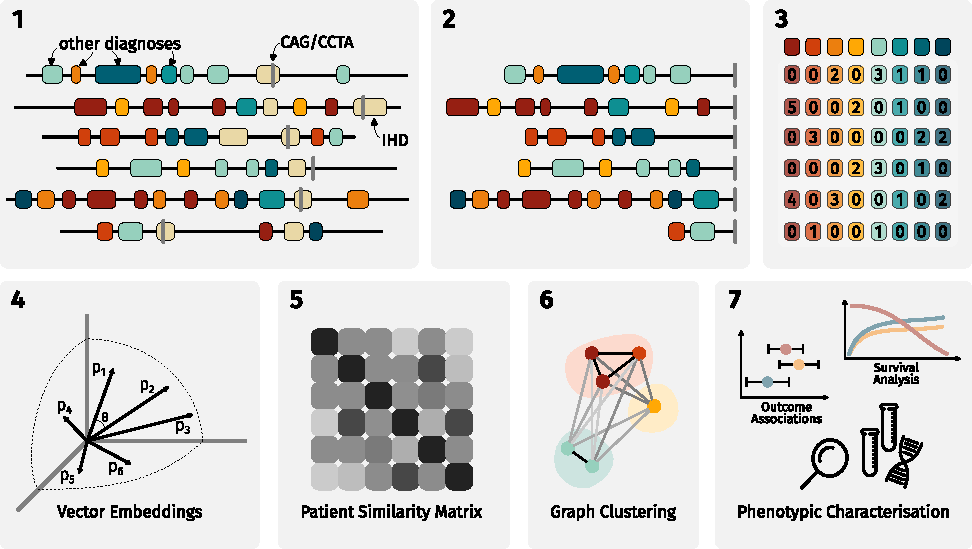
\includegraphics{graphics/clustering-overview.pdf}
    \caption[Overview of the comorbidity clustering approach]{%
        Overview of the comorbidity clustering approach in \studyi{},
        detailing the different steps going from \ac{LPR} patient record data
        to identification and characterisation of distinct 
        multimorbidity clusters. 
    }
    \label{fig:dishisclust}
\end{figure*}

The overall methodology employed in this study is illustrated 
in \cref{fig:dishisclust}. In the following, I will be outlining the 
different steps of our comorbidity clustering approach. 

In this study, we represented multimorbidity by constructing patient-level
vectors that aggregated all diagnosis codes assigned up until the index date 
(as illustrated by steps 1 and 2 in \cref{fig:dishisclust}).
We excluded \ac{IHD} codes (\ac{ICD-10}: I20-25) and
codes belonging from chapters XV, XVI, XVII, XIX, XX, and XXI.%
\sidenote{%→
    These chapters are in the Danish \ac{ICD-10} version defined as
    \begin{itemize}[itemsep=1pt, parsep=0pt]
        \item Chapter XV (O00-O99): Pregnancy, childbirth and the puerperium
        \item Chapter XVI (P00-P99): 
            Certain conditions originating in the perinatal period
        \item Chapter XVII (Q00-Q99):
            Congenital malformations, deformations and chromosomal abnormalities
        \item Chapter XIX (S00-T98): 
            Injury, poisoning and certain other consequences of external causes
        \item Chapter XX (X60-Y09): 
            External causes of morbidity and mortality
        \item Chapter XXI (Z00-Z99): 
            Factors influencing health status and contact with health services
    \end{itemize}
}
% ←
In addition, we removed rarely used codes assigned to less than five patients.

The remaining codes were then counted (step 3), 
and embedded in a vector space model 
~\autocite{saltonVector1975}
using \ac{SVD}
~\autocite{golubSingular1971} (step 4).
Next, we used these embedded patient-level vectors 
to create a patient similarity matrix (step 5). 
For this matrix, we used cosine similarity as the similarity measure,
which calculates the cosine of the angle \(\theta\) 
between the embedded vectors.

From the similarity matrix we could then 
construct a patient similarity network,
which is a weighted undirected graph with 
patients as vertices. 
The edges in the graph represents the connections between patients,
which is weighted by the similarity of their respective diagnosis vectors.
As this graph could contain a total of
\num{2609922876} edges, which is computationally intractable, 
we pruned the network by discarding low-similarity edges 
(\(\cos{\theta} \leq 0.3\)) and limited the number of edges
connected to each vertex to the \num{8000} with greatest weight.

Subsequently,
the patient similarity network,
was then subject to cluster analysis,
using the \ac{MCL} algorithm 
~\autocite{vandongenGraph2008}
(step 6). 
The clusters obtained were then characterised (step 7).
This characterisation involved four key aspects 
(i) estimation of \acp{HR} for cluster comparisons using Cox proportional hazards models,
(ii) phenotypic enrichment analysis, 
(iii) examination of clusters based on laboratory test profiles,
and (iv) testing for genetic associations through \acp{PRS}.
In the following I will limit the presentation
of results to aspects (i) and (ii), 
as these are most integral to the study,
and will otherwise refer to the full-length manuscript.

\section{Main Findings}

% \subsection{Cohort Characteristics}
% 
% The study included \num{72249} patients, 
% predominantly male (\qty{63.1}{\percent}), with a mean age of 63.9
% years. 
% The most common inclusion diagnosis was angina pectoris, followed by acute
% myocardial infarction and chronic IHD. The most common comorbidities recorded
% prior to the index \ac{CAG} or \ac{CCTA} is
% hypertension (I10.9), dyslipidemia (E78.0), 
% and non-insulin-dependent diabetes (E11.9).
% The average number of diagnoses in the patient vectors, i.e. prior to index,
% was \num{8.1}. 
% Of the entire cohort, \qty{6.7}{\percent} had no prior diagnoses registered.

\subsection{Cluster Analysis and Outcomes}

%The clustering identified 36 distinct patient subgroups 
%which in total included \qty{94}{\percent} of the cohort. 
%The patients not belonging to a cluster, 
%was primarily those without any registered diagnoses.
%We discarded clusters with a size less than 500 (4 clusters),
%since the goal was to describe the more general patterns of multimorbidity,
%and instead focused the characterisation to the remaining 31 clusters.

The clustering resulted in 31 distinct patient subgroups, 
each characterised by specific patterns of multimorbidity.
We incorporated cluster membership in Cox regression models, 
which was further adjusted for sex and age. 
This was to obtain estimates for the risk associated with the comorbidity
profiles in each cluster, beyond those patterns primarily dependent on
age or sex.
The \acp{HR} were estimated 
by contrasting each single cluster against all others.
The size of clusters, mean age at index, and average propotion of males, 
and the adjusted \acp{HR} for the two outcomes, are
depicted in \cref{fig:cluster-results}.

\begin{figure*}[t!]% →
    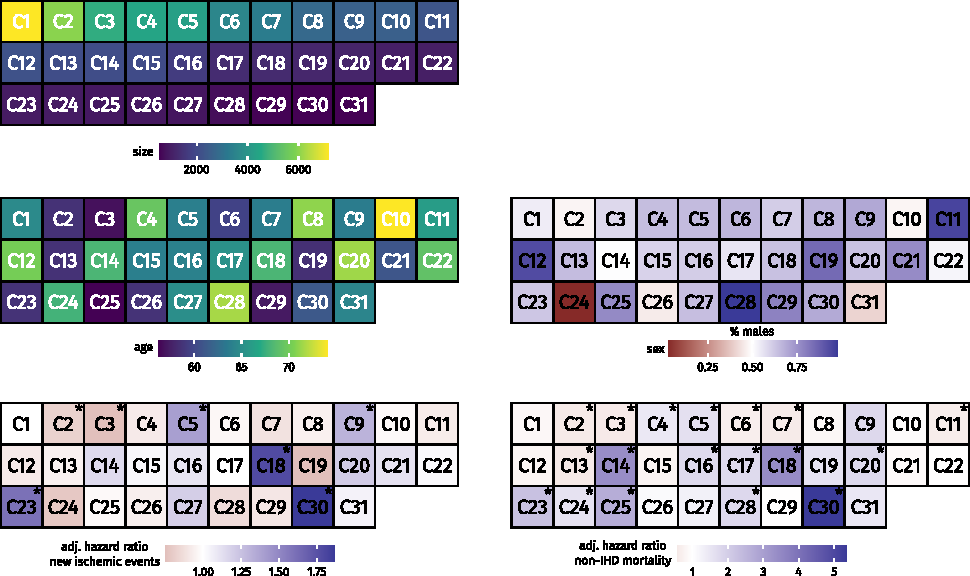
\includegraphics{graphics/clustering-results.pdf}
    \caption[Cluster characteristics and outcomes][0em]{%
        Cluster characteristics and adjusted hazard ratios.
        The first panel,
        from top-left to bottom-right,
        shows the number
        of patients in each cluster, 
        arranged according to their respective sizes.
        This ordering is maintained in subsequent panels.
        The second panel shows the average age at the index \ac{CAG}/\ac{CCTA},
        ranging from \qty{56.2}{years} (C25) to \qty{74.2}{years} (C10).
        The third panel shows the sex distribution in each cluster,
        using fill color to indicate the proportion of males;
        red for clusters with more than \qty{50}{\percent} females,
        and blue for those with more than \qty{50}{\percent} males.
        The fourth and fifth panels shows the adjusted hazard ratios
        for new ischemic events and non-\ac{IHD} mortality, respectively.
        Here, clusters with a red fill indicate an \ac{HR} below one,
        while those with a blue fill have an \ac{HR} above one.
        Clusters with a hazard ratio significantly different from
        one are marked with an asterisk (\(*\)).
    }
    \label{fig:cluster-results}
\end{figure*}% ←

Our analysis revealed that
certain clusters had significantly different risks compared to others.
Comorbidity profiles within five clusters (C5, C9, C18, C23, C30) were
associated with a significantly increased risk of new ischemic events.
Conversely, profiles in two clusters (C2, C3) were associated with a 
significantly reduced risk of these events. 
Twelve clusters (C4, C5, C14, C16, C17, C18, C20, C23, C24, C25,
C28, C30) had profiles associated with a significantly higher risk 
of non-\ac{IHD} mortality. 
In contrast, six clusters (C2, C3, C6, C7, C11, C13) had
profiles that were linked to a significantly lower risk of 
non-\ac{IHD} mortality.
Of note, four of the five cluster profiles with an increased risk of 
new ischemic events also exhibited an increased risk of 
non-\ac{IHD} mortality. 

\subsection{Phenotypic Characterisation of Clusters}

\begin{figure*}[tbp]% →
    \includegraphics[clip=false, trim=6mm 5mm 0 4mm]%
        {graphics/cluster-summary.pdf}
    \caption[Overview of cluster phenotypes]{%
        From manual review of the between-cluster enrichment of 
        diagnosis codes, we assigned each cluster a label based
        on its most prevalent codes.
        To aid the intrepretation, the clusters were further organized by 
        consideration of their estimated hazard ratios 
        and shared diagnostic similarity.
        Clusters marked with \uporange{} or \upblue{} have a 
        significantly increased risk of new ischemic events
        and non-\ac{IHD} mortality, respectively.
        Conversely, \downorange{} or \downblue{} marks those with
        a significantly decreased risk.
        A single arrow indicates the direction of the effect 
        and that the association was not found to be significant.

    }
    \label{fig:cluster-summary}
\end{figure*}% ←

% To describe the patterns associated with increased or 
% decreased risks, we further characterised the clusters
% and summarise our key findings here.

As a first step, we evaluated the intra-cluster prevalence of all unique diagnosis
codes (\num{3046} in total) within patient vectors. 
These prevalences was then compared with the average prevalences
across all clusters by calculating \ac{OE}-ratios, 
to pinpoint \ac{ICD-10} codes that were disproportionately represented 
in various clusters.  
The top ten most overrepresented or underrepresented codes for each
cluster are detailed in supplementary tables 5A and 5B of the manuscript
(\cref{chap:study1-paper}).

We conducted a manual review of these findings, assigning a label to each
cluster based on the associated codes. Given that multiple codes could pertain
to a single cluster, these labels are not definitive but offer a general
overview, as depicted in \cref{fig:cluster-summary}. 
Furthermore, in \cref{fig:cluster-summary}, we organise the
clusters by both their common traits and the hazard ratios 
derived from the Cox analyses.

\section{Interpretation}

From \cref{fig:cluster-summary}, 
we see that the five clusters (C5, C9, C18, C23, C30) with a 
significantly increased risk of both new ischemic events and non-\ac{IHD} mortality
were characterised by the presence of important prognostic comorbidities in \ac{IHD}:
diabetes, peripheral atherosclerosis, heart failure, 
and chronic kidney disease. 

Both diabetes and chronic kidney disease 
are highlighted as important non-cardiovascular
comorbidities in the 2019 \acsu{ESC} guidelines for chronic coronary syndromes,
and both peripheral artery disease and renal dysfunction is explicitly
described as comorbidities that negatively impact prognosis.%
\sidecite[15em]{knuuti20192020}
Heart failure, 
also known to affect prognosis and included in clinical guidelines,
is, for example, included as one of eight carefully selected predictors
in the widely used \acsfont{GRACE} risk and mortality calculator.%
\sidecite[13em]{foxShould2014}
This showcases that our framework is able to identify known comorbidites
that affect the clinical course of cardiovascular disease.
In addition, it further emphasizes the significance of these 
comorbidities and the broader concept of considering
comorbidity in clinical assessment of \ac{IHD}.

We did not identify other clusters with comorbidity profiles
that significicantly increased the risk of new ischemic events,
however, both the second and third largest clusters (C2 and C3)
were found to have comorbidities associated with a significant decreased risk
of both new ischemic events and non-\ac{IHD} mortality.
Cluster C2 is characterised by the presence of codes 
for both gallstones (K80) and abdominal pain (R10).
Cluster C3 relates to symptom codes (R00-R99),
with high \ac{OE}-ratios for
{pain in throat and chest} (R07.9), 
{other chest pain} (R07.3), 
and {muscle strain} (M62.6).

It is interesting that the second largest cluster (C2)
is characterised by gallstones as a comorbid condition.
Many studies have previously reported a link between
gallstones and ischemic heart disease,
\autocite{zhengGallstones2016}
\autocite{upalaGallstone2017}
\autocite{wirthPresence2015}
however, the underlying reasons for this association remain
somewhat unclear and it is uncertain the link is causal.
It is known that the two diseases shares pathogenicity factors,
which include hypercholesterolemia, diabetes, and hypertension,
so parts of the pathological mechanism is likely shared.
\autocite{zhengGallstones2016}

In our study, focusing on patients with incident \ac{IHD},
the presence of gallstones appear to positively affect prognosis.
A possible explanation is that acute symptoms of gallstone disease
can immitate heart disease symptoms, and thus, the cluster could be 
enriched for patients that may not have \ac{IHD} to begin with.
This area warrants further investigation to better understand these connections
and their implications for clinical practice.

Two clusters were characterised by the co-occurence of cancer comorbidities.
Clusters C24 and C28 were enriched for breast and prostate cancer, 
respectively.
Our current methodology does not distinguish between active cancer
or if the patient has been cured, which represents a key limitation
of the approach.
However, both clusters were found to have an increased risk of 
non-\ac{IHD} mortality.

In patients with active cancer,
the management of \ac{IHD}, and specifically \ac{ACS}, 
is challenged by increased risk of bleeding,
low platelet count, and increased thrombotic risk.
~\autocite{byrne20232023}
Furthermore, 
many chemotherapeutic agents have cardiotoxic side effects,
as discussed in a 2016 \ac{ESC} position paper on the 
cardivascular toxicity of cancer treatment.
~\autocite{zamorano20162016}
Moreover,
studies indicate that radiotherapy breast cancer
is associated with an increased risk of developing \ac{IHD}, 
in a dose-dependent manner.
~\autocite{darbyRisk2013}
This underscores the complex balancing act involved in concurrently managing
both conditions, where the treatment of one disease can potentially exacerbate
the other.

\section{Conclusion}

In this study, we presented a large-scale data-driven approach
for analysis of comorbidity patterns in more than \num{70000} adult 
patients with incident \ac{IHD}.
We took a hypothesis-free approach and used a broad definition of 
multimorbidity, including more than \num{3000} different \ac{ICD-10} codes in
the decription of prior and coexisting comorbidities in \ac{IHD}.
Using unsupervised clustering, we identified disctinct groups of patients 
each characterised by specific patterns of multimorbidity and associated
risks of both disease progression and mortality from unrelated causes.

Using this approach, we were able to identify clusters characterised by
the presence of well-established prognostic comorbidities, including
diabetes, peripheral atherosclerosis, heart failure, and chronic kidney
disease. 
All clusters associated with these diseases
were all found to be significantly associated with an 
increased risk of adverse events. 
These findings thus represents a form of positive control
which supports the validity of the described methodology.

It is important to emphasize that the presented clustering is not
intended to provide the definitive or universally applicable 
multimorbidity subgroups in \ac{IHD}. 
Instead, the purpose and implication is to provide a valuable tool
for the data-driven exploration of real-world multimorbidity patterns
in \ac{IHD}.
As such, it can be used for generating hypotheses and can likely inform
and guide future research on multimorbidity-informed
treatment and management of \ac{IHD}.

Mapping out the landscape of multimorbidities in a real-world cohort of 
patients with \ac{IHD}, could inform clinical managment and could serve
as a tool for identification of comorbidity combinations for which
current clinical knowledge is currently limited.
Strict inclusion and exclusion criteria in many \acp{RCT} 
potentially limit the applicability of existing \ac{IHD} 
management guidelines on patients with pronounced multimorbidity.
~\autocite{richKnowledge2016}
To adress such limitations, an important first step is to obtain an overview
of the specific patterns of multimorbidity associated with \ac{IHD}.
 
\chapter{Study II: Time-to-Event Prediction of All-Cause Mortality}
\label{chap:study2-outline}


In this large prospective cohort study,
we developed a neural network-based survival model
for prediction of all-cause mortality in patients with \ac{IHD}.
The model was built using real-world data from more than \num{40000} patients
with more than \num{400} different features.


First, our machine learning model significantly improved the predicitive
performance compared to the established \ac{GRACE} 2.0 risk-prediction model.
Second, we showed that utilising and integrated a broad array of features
gives significant better performance than limiting the feature set to only
a single modality or a select handfull of established risk factors.


 
\chapter{Study III: Time-to-Event Prediction with Competing Risks}
\label{chap:study3-outline}

In this chapter, I provide an outline of our research in \studyiii{}.
The manuscript, titled \enquote{%
    Development of a neural network-based competing risk model for long-term
    prognostication in ischemic heart disease from a large database of
    electronic health records and clinical registries},
is currently work in progress, 
and thus the version included in \cref{chap:study3-paper} is 
a draft manuscript.

\section{Background and Aims}

In our previous study, \studyii{}, we demonstrated that a \ac{ML} based 
time-to-event prediction algorithm can improve the prediction of all-cause
mortality in patients with \ac{IHD}. 
While all-cause mortality is an important clinical outcome, 
a limitation of our previous work was the absence of more
disease-specific outcomes such as cardiovascular mortality
and disease progression events.
The neural network-based Logistic-Hazard model employed in \pmhnet{1}
is not able to model competing risks, which precluded the inclusion
of such outcomes.

To address this shortcoming, and further expand on our prior work,
the primary goals of this study are to develop and implement an extension 
to the discrete time Logistic-Hazard model from \textcite{gensheimerScalable2019} 
to enable joint-modelling of competing risks,
and then use our novel framework in the creation of \pmhnet{2}, 
such that it is possible differentiate between deaths related to 
\ac{IHD} and those arising from completely unrelated causes,
in addition to predicting specific measures of disease progression.

\section{The Logistic-Hazard Approach for Competing Risks}

In the following, I will outline how the discrete-time framework can 
be extended to allow for jointly modelling time-to-event data with competing
risks. The theory underlying this approach is well-established in
classical statistical literature, as exemplified by \textcite{tutzModeling2016}, 
but have to the best of our knowledge not yet been adapted to 
neural network models. 

As delineated in \cref{sec:disctime-survival}, 
in the discrete-time framework, 
continuous follow-up time \(\Tic\) is divided into \(q\) contiguous intervals
%
\begin{equation*}
	(0, a_1], (a_1, a_2], \dots, (a_{q-1}, a_q]
\end{equation*}
%
and \(\Tid \in \{1, \dots, q\}\) is then a discrete random variable 
specifying the event time that refers to each interval 
\((a_{\tid-1}, a_{\tid}]\), and similarly, \(\Cid \in \{1, \dots, q\}\)
specifies the time of censoring.

In this framework, a right-censored survival dataset 
\(\mathfrak{D}_{\mathrm{d}}\) with \(\kappa\) different competing 
risks is defined as
\begin{equation}
    \mathfrak{D}_{\mathrm{d}} = 
        \{(\tid_i, \sigma_i, \vec{x}_i) \mid i = 1, \ldots, N\} 
\end{equation}
where \(t_i = \min(T_{i}, C_i)\) is the observed follow-up time,
\(\sigma_i \in \{\varnothing, 1, \dots, \kappa\}\) is the event indicator 
(with \(\varnothing\) specifying censored observations),
and \(\vec{x}_i \in \mathbb{R}^{p}\) is a feature vector of size \(p\).

\subsection{Model Formulation}

For modelling this data, we use the discrete 
cause-specific hazard, which for cause \(r\) is defined as
~\autocite{tutzModeling2016}
\begin{equation}
    \label{eq:cause-specific-hazard}
    \lambda_r(t \giv \vec{x}) = 
    \Pr(\Tid = \tid, R = r \mid \Tid \geq \tid, \vec{x}).
\end{equation}
This hazard describes the conditional probability of experiencing event \(r\) 
in the interval \((a_{\tid-1}, a_{\tid}]\) given that the individual
is still at risk at the beginning of the interval.

For \(\kappa\) competing risks, the survival data can be described with
\(\kappa\) different hazard functions, 
\(\lambda_{1}(\tid \giv \vec{x}), \dots, \lambda_{\kappa}(\tid \giv \vec{x})\).
To describe the overall hazard \(\lambda(\tid \giv \vec{x})\), 
these functions can be combined as
~\autocite{tutzModeling2016}
\begin{equation}
    \label{eq:overall-hazard}
    \lambda(\tid \giv \vec{x}) 
    = \sum_{r=1}^{\kappa} \lambda_{r}(\tid \giv \vec{x})
    = \Pr(\Tid = \tid \mid \Tid \geq \tid, \vec{x}),
\end{equation}
which describes the risk of experiencing any of the competing risks.

From \cref{eq:overall-hazard}, we can obtain the survival function,
which describes the probability of not experiencing any of the competing
risks.

\begin{equation}
    S(\tid \mid \vec{x}) = \Pr(\Tid > \tid \mid \vec{x}) 
    = \prod_{s=1}^{\tid} (1 - \lambda(s \giv \vec{x}))
\end{equation}


At each interval \((a_{\tid-1}, a_{\tid}]\), 
there are \(\kappa + 1\) different possible outcomes,
either one of the \(\kappa\) risks occurs
or the individual survives and continues to the next interval,
which means that the sum of these probabilities is 1.
\begin{equation}
    \lambda_{1}(\tid \giv \vec{x}) 
    + \dots
    + \lambda_{\kappa}(\tid \giv \vec{x})
    + (1 - \lambda(\tid \giv \vec{x}))
    = 1
\end{equation}

To model these \(\kappa + 1\) events,
we construct a neural network where the output is
a \(N \times q \times (\kappa + 1)\) matrix of \enquote{logits}%
\sidenote{In the context of machine learning,% →
the term \enquote{logits} typically refers to 
the raw unnormalized output that can range from \(-\infty\) to \(\infty\).
To obtain probabilities from logits, they are passed through an 
activation function such as the logistic or \(\mathrm{Softmax}\) function}
% ←
as illustrated in \cref{fig:ext-loghaz}.
To obtain outputs on the probability scale,
the logits are passed through a Softmax activation function,
such that the numbers across the dimension of the probability matrix 
sum to 1.

The \(1 - \lambda(\tid \giv \vec{x})\) term is not strictly necessary 
to include, since it can be obtained from the others, 
however in the machine learning literature it is common practice to include all 
output classes in multinomial predictions. In the following, 
I will refer to this term as \(\lambda_\varnothing(\tid \giv \vec{x})\).

\begin{marginfigure}% →
\begin{tikzpicture}% →
    \useasboundingbox (-.5,-0.5) rectangle (6.8, 5.6);
    \begin{scope}[transform canvas={scale=.65}]

    \draw[->] (5.3,    0) -- ( 7.1,  1.6) node[below, midway, sloped, font=\large] {events};
    \draw[->] (0,   -0.3) -- ( 5.0, -0.3) node[below, midway, sloped, font=\large] {time};
    \draw[->] (-0.3, 4.0) -- (-0.3,  0.0) node[below, midway, sloped, font=\large] {batch};

    \begin{scope}[xshift=1.8cm, yshift=1.6cm]
         \renewcommand{\y}[1]{\lambda_{#12}}
         \fill[white,fill opacity=.9] (0,0) rectangle (5, 4);
         \draw[step=1cm, black, very thin] (0,0) grid (5, 4);
         \matrix[matrix of nodes, 
             inner sep = 0pt, outer sep = 0pt,
             matrix anchor=south west,
             nodes={minimum width=1cm, anchor=center, minimum height=1cm, 
                    outer sep=0pt, inner sep=0, align=center, font=\large},
             column sep=0em, row sep=0em
        ]  at (0, 0)
         {
             $\y{11}$  & $\y{12}$ & $\y{13}$ & $\dots$  & $\y{1j}$  \\
             $\y{21}$  & $\y{22}$ & $\y{23}$ & $\dots$  & $\y{2j}$  \\
             $\vdots$  & $\vdots$ & $\vdots$ & $\ddots$ & $\vdots$  \\
             $\y{i1}$  & $\y{i2}$ & $\y{i3}$ & $\dots$  & $\y{ij}$  \\
         };
    \end{scope}
    
    \begin{scope}[xshift=.9cm, yshift=.8cm]
         \renewcommand{\y}[1]{\lambda_{#11}}
         \fill[white,fill opacity=.9] (0,0) rectangle (5, 4);
         \draw[step=1cm, black, very thin] (0,0) grid (5, 4);
         \matrix[matrix of nodes, 
             inner sep = 0pt, outer sep = 0pt,
             matrix anchor=south west,
             nodes={minimum width=1cm, anchor=center, minimum height=1cm, 
                    outer sep=0pt, inner sep=0, align=center, font=\large},
             column sep=0em, row sep=0em
        ]  at (0, 0)
         {
             $\y{11}$  & $\y{12}$ & $\y{13}$ & $\dots$  & $\y{1j}$  \\
             $\y{21}$  & $\y{22}$ & $\y{23}$ & $\dots$  & $\y{2j}$  \\
             $\vdots$  & $\vdots$ & $\vdots$ & $\ddots$ & $\vdots$  \\
             $\y{i1}$  & $\y{i2}$ & $\y{i3}$ & $\dots$  & $\y{ij}$  \\
         };
    \end{scope}

    \begin{scope}
         \renewcommand{\y}[1]{\lambda_{#10}}
         \fill[white,fill opacity=.9] (0,0) rectangle (5, 4);
         \draw[step=1cm, black, very thin] (0,0) grid (5, 4);
         \matrix[matrix of nodes, 
             inner sep = 0pt, outer sep = 0pt,
             matrix anchor=south west,
             nodes={minimum width=1cm, anchor=center, minimum height=1cm, 
                    outer sep=0pt, inner sep=0, align=center, font=\large},
             column sep=0em, row sep=0em
        ]  at (0, 0)
         {
             $\y{11}$  & $\y{12}$ & $\y{13}$ & $\dots$  & $\y{1j}$  \\
             $\y{21}$  & $\y{22}$ & $\y{23}$ & $\dots$  & $\y{2j}$  \\
             $\vdots$  & $\vdots$ & $\vdots$ & $\ddots$ & $\vdots$  \\
             $\y{i1}$  & $\y{i2}$ & $\y{i3}$ & $\dots$  & $\y{ij}$  \\
         };
    \end{scope}
    \end{scope}
\end{tikzpicture}
% ←
\caption[Illustration of the extended Logistic-Hazard model]{
    The output of the extended Logistic-Hazard model is a
    \(N \times q \times (\kappa + 1)\) matrix of logits, which 
    represents the cause-specific hazards.}
\label{fig:ext-loghaz}
\end{marginfigure}% ←

\subsection{Derivation of Loss Function}
\newcommand{\lambdanull}[1]{\lambda_\varnothing(#1 \giv \vec{x}_i)}

As detailed in \textcite{tutzModeling2016}, 
the contribution of 
the \(i\)th individual on the likelihood is
%
\begin{equation}
    \Lik_{i} =
    \begin{cases}
        \Pr(\Tid = \tid_{i}, R = \sigma_i \mid \vec{x}_i) 
        \Pr(\Cid \geq \tid \mid \vec{x}_i) 
        & \text{if non-censored} \\
        \Pr(\Tid > \tid_{i} \mid \vec{x}_i) 
        \Pr(\Cid = \tid \mid \vec{x}_i)                  
        & \text{if censored.}
    \end{cases}
\end{equation}

Assuming that censoring is non-informative, 
the probabilities involving the censoring time \(\Cid\) can be omitted.
~\autocite{tutzModeling2016}
Further, we can rewrite the terms 
\(\Pr(\Tid = \tid_{i}, R = \sigma_i \giv \vec{x}_i)\) and 
\(\Pr(\Tid > \tid_{i} \giv \vec{x}_i) \) 
as a product of the conditional hazards
\begin{align}
\begin{split}
    \Pr(\Tid = \tid_{i}, R = \sigma_i \mid \vec{x}_i) 
    &= 
    \PR (\Tid = \tid_{i}, R = \sigma_{i} \mid \Tid \geq \tid_{i}, \vec{x}_i) 
    \PR (\Tid  \geq \tid_i \mid \vec{x}_i) \\
    &= \lambda_{\sigma_i}(\tid_i \giv \vec{x}_i) \PR (\Tid  > \tid - 1 \mid \vec{x}_i) \\
    &= \lambda_{\sigma_i}(\tid_i \giv \vec{x}_i) \, 
    \textstyle \prod_{s=1}^{\tid_i - 1} (1 - \lambda(s \giv \vec{x}_i)) \\
    &= \lambda_{\sigma_i}(\tid_i \giv \vec{x}_i) \, 
    \textstyle \prod_{s=1}^{\tid_i - 1} \lambda_\varnothing(s \giv \vec{x}_i)
    \raisetag{2em}
\end{split} \\
\begin{split}
    \Pr(\Tid > \tid_{i} \giv \vec{x}_i) 
    &= 
    \PR (\Tid > \tid_{i} \mid \Tid \geq \tid_{i}, \vec{x}_i) 
    \PR (\Tid  \geq \tid_i \mid \vec{x}_i) \\
    &= 
    (1 - \PR (\Tid = \tid_{i}  \mid \Tid \geq \tid_{i}, \vec{x}_i)) 
    \PR (\Tid  > \tid_i - 1 \mid \vec{x}_i) \\
    &= (1 - \lambda(\tid_i \giv \vec{x}_i)) \, 
    \textstyle \prod_{s=1}^{\tid_i - 1} (1 - \lambda(s \giv \vec{x}_i)) \\
    &= \textstyle \prod_{s=1}^{\tid_i} \lambda_\varnothing(s \giv \vec{x}_i)
    \raisetag{2em},
\end{split} 
\end{align}
and the likelihood contribution is then

\begin{equation}
    \Lik_{i} =
        \lambda_{\sigma_i}(\tid_i \giv \vec{x}_i) \, 
        \prod_{s=1}^{\tid_i - 1} \lambda_\varnothing(s \giv \vec{x}_i)
\end{equation}

To avoid computational issues with floating point precision, 
we use the log-likelihood instead, which becomes
\begin{equation}
    \lik_{i} =
        \log [\lambda_{\sigma_i}(\tid_i \giv \vec{x}_i)] +
        \sum_{s=1}^{\tid_i - 1} \log [\lambdanull{s}]
\end{equation}

The total log-likelihood of all datapoints gives the loss-function
used in the extended Logistic-Hazard model for competing risks,
which is
\begin{equation}
    \label{eq:lhx-loglikelihood}
    \lik(\mathfrak{D}_{\mathrm{d}}) = 
        \sum_{i = 1}^{N} \left(
        \log [\lambda_{\sigma_i}(\tid_i \giv \vec{x}_i)] +
        \sum_{s=1}^{\tid_i - 1} \log [\lambdanull{s}]
        \right)
\end{equation}

\subsection{Implementation}

This loss function, along with several useful classes and functions 
for discrete time-to-event neural networks, have been implemented in
the python package \texttt{DiscoTime}.
~\autocite{holmDiscotime}
This implementation relies on the \texttt{PyTorch} machine learning framework
and is built to use the \texttt{PyTorch-Lightning} interface, to make
protyping and experimentation as easy as possible.
\texttt{DiscoTime} is available on the \ac{PyPI} and on 
GitHub at \enquote{peterchristofferholm/discotime}.
Currently in early development, the documentation is rather limited 
and the code base is expected to undergo re-factorization, 
but we still expect that the framework in its current state
is of general interest to other researchers in the field.
We used version 0.1.0 of the package for this study.

\section{Study Design and Methodology}

\begin{marginfigure}[0em]% →
    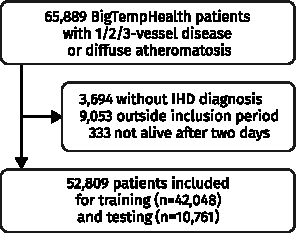
\includegraphics{graphics/pmhnet-v2-inclusion-flowchart.pdf}
    \caption[Inclusion diagram for \pmhnet{2}]{%
        Flow diagram showing the inclusion and exclusion criteria 
        for derivation of thè \pmhnet{2} cohort. An \acs{IHD} diagnosis
        was defined as any prior or concurrent hospital admission with 
        a primary or secondary diagnosis code (\acs{ICD-10}) of I20-25.
        The inclusion period ranged from 01.01.2006 to 31.12.2016, 
        both dates inclusive.}
    \label{fig:pmhnet-v2-inclusion}
\end{marginfigure}
% ←

To test the utility of the presented competing risk methodology,
we set out to develop \pmhnet{2}, a collection of four different 
neural network-based time-to-event prediction models for cause-specific 
post-angiography prognostication in \ac{IHD}.

\subsection{Defining the Derivation Cohort}

For development of the neural network models, 
we linked the \ac{BTH} dataset to 
the \ac{LPR} and the \ac{EDHR}.
From these, 
we identified patients who underwent a \ac{CAG} which led to a diagnosis of
one-, two-, or three-vessel disease or diffuse atheromatosis between January 1,
2006, and December 31, 2016.
Patients were excluded if they lacked an
\acsu{ICD-10} code for \ac{IHD} (I20-25),
were under 18 years at the time of the \ac{CAG},
or did not survive at least two days after the index procedure
(\cref{fig:pmhnet-v2-inclusion}).

\begin{marginfigure}[0em]% →
    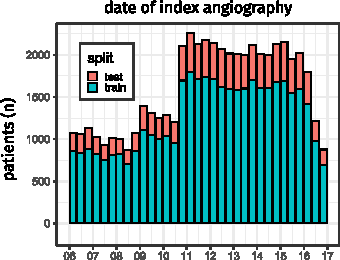
\includegraphics[trim=5mm 0 0 0]{graphics/pmhnet-v2-inclusion-histogram.pdf}
    \caption[Distribution of \pmhnet{2} inclusion times]{%
    Histogram showing the temporal distribution of the \pmhnet{2} index
    coronary angiography procedures. 
    The bars represent the number of patients with an index event in each
    four-month period from 2006 to 2017,
    further segmented to display the proportions of train and test patients.}
    \label{fig:pmhnet-v2-histo}
\end{marginfigure}
% ←

This cohort consists of \num{52809} adults with \ac{IHD}, 
closely resembling and considerably overlapping  
the one used in the \pmhnet{1} study (\studyii{}).
However, unlike \pmhnet{1}, 
which only included 
patients undergoing their first \ac{CAG} 
during the inclusion period,
this study expanded the criteria to 
also include patients with a history of one or more \acp{CAG}.
This approach likely provides 
a more comprehensive representation 
of the diverse manifestations of chronic coronary syndromes.

Prior to statistical analysis and  model training, 
each patient in the development cohort was randomly allocated to the 
training or test split with probabilities of 
\qty{80}{\percent} and \qty{20}{\percent}, 
respectively.
This process resulted in 
a training set of \num{42048} patients 
and a test set of \num{10761} patients
(\cref{fig:pmhnet-v2-histo}).

Serving as model predictors,, 
we identified and created more than 2200 different
features belonging to five different overall categories.
We included 80 clinical features, 418 procedure and examination codes,
785 distinct medical prescriptions, 504 different diagnoses, 
and 475 unique laboratory test features.
Further details on features and the pre-processing 
is included in the manuscript in \cref{chap:study3-paper}.

\subsection{Included Time-to-Event Endpoints}

As the index date, we used the date of the inclusion \ac{CAG}.
For the \pmhnet{2} time-to-event prediction models, 
follow-up was defined as the number of days 
between the index date and the onset of endpoints or censoring,
whichever came first, 
with a maximum follow-up duration of five years.
We defined four different primary outcomes, 
three of which included competing risks:

\begin{marginfigure}[2em]% →
    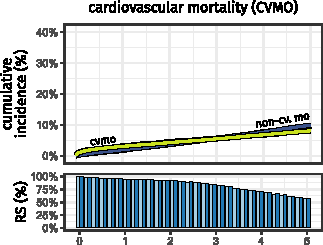
\includegraphics[trim=5mm 0 0 0]{graphics/pmhnet-v2-cvmo-cic.pdf}
    \caption[Cumulative incidence of the \acsfont{CVMO} outcome]{%
        Cause-specific cumulative incidence functions for the 
        \acsfont{CVMO} outcome (cvmo) and the competing endpoint 
        \enquote{non-cardiovascular} mortality. (non-cv. mo). 
        The bottom panels shows the proportion of train/test patients
        still at risk (i.e. non-censored and still alive) 
        at each two-month period following the index \acs{CAG}.}
    \label{fig:pmhnet-v2-cic}
\end{marginfigure}
% ←

\begin{description}
    \item[\acsfont{ACMO}---all-cause mortality,]
        was obtained from the \ac{CPR}
        using the same definition as in \studyii{}.
        \acsfont{ACMO} did not have competing risks.

    \item[\acsfont{CVMO}---cardiovascular mortality,]
        was defined from the \ac{DAR} as deaths where the underlying
        cause of death was assigned an \ac{ICD-10} code from the 
        cardiovascular chapter (I00--99).
        Deaths attributed to different causes  were 
        treated as competing risks, as depicted in \cref{fig:pmhnet-v2-cic}

    \item[\acsfont{CVCO}---cardiovascular complications,] 
        was defined from the \ac{LPR} as a composite outcome 
        covering hospital admissions with a primary diagnosis of
        \enquote{heart failure} (\acs{ICD-10}: I50),
        \enquote{atrial fibrillation or flutter} (I48),
        \enquote{cardiac arrest} (I46),
        and 
        \enquote{cerebrovascular accident} (I61, I63--64)
        and in-hospital procedures for 
        \enquote{implanation of pacemaker} (\acs{SKS}: \texttt{"BFCA0*"})
        and
        \enquote{implanation of cardioverter-defibrillator} (\texttt{"BFCB0*"}).
        Events within four weeks after the index angiography was assumed
        to be unrelated to disease progression and was ignored.
        \acsfont{ACMO} was treated as a competing risk.

    \item[\acsfont{MIEV}---new myocardial ischemia,] 
        was defined from the \ac{LPR} as 
        unplanned \acp{PCI}, \acp{CABG}, or 
        in-hospital admissions longer than \qty{24}{\hour}
        with a primary diagnosis of \ac{IHD} (I20-25).
        Events within the eight weeks after the index \ac{CAG} 
        were not considered \enquote{new} events 
        and were therefore excluded.
\end{description}

\subsection{Neural Network Architecture}

For the \pmhnet{2} models, 
we used a \enquote{ResNet}-inspired neural network architecture
adapted for tabular data, as advocated by \textcite{gorishniyRevisiting2023}.
This architecture consists of multiple so-called residual blocks,
or \enquote{ResBlocks}, sequentially connected to one another.
For \pmhnet{2}, these ResBlocks were defined as
%
\begin{equation}
    \mathrm{ResBlock}_{h}(z) = ( 
    \mathrm{BN} 
    \circ \mathrm{FC}_{h,h} 
    \circ \mathrm{DO} 
    \circ \mathrm{SiLU} 
    \circ \mathrm{FC}_{h,h} 
    \circ \mathrm{DO} 
    )(z)  + z
\label{eq:resblock}%
\end{equation}%
where \(\mathrm{BN}\) is a batch normalization function,
\(\mathrm{FC}_{h,h}\) is a fully-connected linear function
with \(h\) inputs and \(h\) outputs, 
\(\mathrm{DO}\) is a dropout function for regularization,
and \(\mathrm{SiLU}\) is the sigmoid-weighted linear unit (\acsfont{SiLU})%
---a non-linear activation function.
~\autocite{elfwingSigmoidWeighted2017}
An important aspect of the ResBlock is the skip-connection,
\(f(z) + z\), where a learned representation is added on top of 
the untransformed input, which can enable training of
very deep neural networks.
~\autocite{orhanSkip2018}
For the models tested, we constrained all ResBlocks to have the same
number of hidden units \(h\) in each of the hidden layers.

By stacking together several of these building blocks,
we can adjust the depth and complexity of the final architecture
\begin{equation}
    \mathrm{ResNet}(z) = 
    (
    \mathrm{FC}_{m,h} 
    \circ 
    \mathrm{ResBlock}_{h} 
    \circ \dots 
    \circ \mathrm{ResBlock}_{h} 
    \circ \mathrm{FC}_{h,o} 
    )(z)
\end{equation}
which depends on the number of input features \(m\),
the number of hidden units \(m\), 
and the number of output logits \(o\).%
\sidenote{%
    Which for our discrete-time competing risk setup is 
    \(q \cdot (\kappa + 1)\), where \(q\) is the number of time bins
    and \(\kappa\) is the number of competing risks.
}

\section{Model Training and Hyperparameter Tuning}

For training neural network models, 
we utilized the \enquote{super-convergence} training protocol
described by \textcite{smithSuperConvergence2018a},
a general methodology for fast and efficient training of
neural network models.
In this approach, 
models are trained for a pre-specified number of steps
using the \enquote{AdamW} stochastic optimization algorithm,
~\autocite{loshchilovDecoupled2019}
and the learning-rate is continuously adjusted during training
following a one-cycle learning rate policy.
We used the \texttt{OneCycleLR} implementation 
from the \texttt{PyTorch} library.%
\sidecite[0em]{paszkePyTorch2019}

Given the multitude of settings that needs to be specfied
for configuration of both the neural network models and
the training process itself, 
we conducted several \ac{HPO} experiments to
explore various combinations of hyperparameters.
For this purpose, we further subdivided the training data
into a training and validation split.
This validation split was used to assess model performance
of the models constructed during the hyperparameters sweeps.
The following gives an overview of the hyperparameters
included in the \ac{HPO}, and the range of possible values explored.

\begin{fullwidth}
\begin{multicols}{3}
\raggedcolumns

We included five parameters to adjust the architecture of the networks
and the complexity of the discretization grid:
\begin{enumerate}[label=\alph*)]
    \item \verb|n_timebins|:
        number of time bins in the discretization grid.
        Allowed values are 
        \numrange{1}{100}.
    \item \verb|n_hidden|:
        number of hidden units in each hidden layer.
        Controls the width of the neural network.
        Allowed values are 
        \numrange{10}{100}.
    \item \verb|n_blocks|:
        number of residual blocks.
        Controls the depth of the neural network.
        Allowed values are 
        \numrange{1}{20}.
    \item \verb|enable_skipconn|:
        should the skip-connection part of the ResBlock
        (\cref{eq:resblock}) be included? 
        Toggle between true/false.
    \item \verb|enable_batchnorm|:
        should the batch-normalization layer of the ResBlock
        (\cref{eq:resblock}) be included? 
        Toggle between true/false.
\end{enumerate}

Four parameters were used to configure the model training process
and to regulate the amount and type of regularization.
\begin{enumerate}[label=\alph*), resume]
    \item \verb|n_step|:
        number of training epochs.
        Range: \numrange{5}{25}.
    \item \verb|max_lr|:
        maximum learning rate in the one-cycle scheduler.
        Range: \numrange{1e-3}{1}.
    \item \verb|weight_decay|:
        amount of  weight decay used in the \verb|AdamW| optimizer.
        Range: \numrange{1e-5}{1}.
    \item \verb|dropout|:  
        dropout rate. 
        Range: \qtyrange{0}{90}{\percent}.
\end{enumerate}

Finally, four parameters controlled the upper limit on the inclusion of 
retrospective data for various features categories, namely:
\begin{enumerate}[label=\alph*), resume]
    \item \verb|cutoff_bioc|: 
        inclusion window for
        laboratory tests results.
        Range: \numrange{0.5}{5},
        stepsize: \num{0.5} .
    \item \verb|cutoff_diag|:
        inclusion window for
        diagnosis codes.
        Range: \numrange{0.5}{10},
        stepsize:  \num{0.5} .
    \item \verb|cutoff_proc|:
        inclusion window for
        procedure and examination codes.
        Range: \numrange{0.5}{10},
        stepsize: \num{0.5} .
    \item \verb|cutoff_medi|:
        inclusion window for
        drug prescription features.
        Range: \numrange{0.5}{10},
        stepsize: \num{0.5} .
\end{enumerate}
    
\end{multicols}
\end{fullwidth}

The \ac{HPO} process was automatized using the \verb|Optuna| framework.
~\autocite{akibaOptuna2019}
As the tuning parameter,
we used the \ac{IPA} of the primary outcome 
(\acsfont{ACMO}, \acsfont{CVMO}, \acsfont{CVCO}, and \acsfont{MIEV}).
Since the \ac{IPA} is a time-dependent measure,
we calculated the \ac{IPA} at 50 evenly spaced timepoints from
\numrange{0.5}{5} years and numerically integrated the values
to provide a single performance measure for the \ac{HPO}. 

After \ac{HPO}, 
we used the best performing configuration for each outcome
and trained the final models on the entire training data.

\subsection{Model Evaluation}

For evaluation of the \pmhnet{2} time-to-event prediction models,
we assessed model discrimination and calibration. 
Similar to \studyii{}, we used \ac{tdAUC} to quantify the models'
cause-specific ability to discriminate between cases and non-cases.
For quantification of model calibration,
we computed the Brier score and the \ac{IPA}. 

The \ac{IPA},
which is an \(R^{2}\)-type measure of model accuracy,
is obtained by scaling the Brier score 
of the model with that of a covariate-less null model 
based on the estimated incidences from the Kaplan-Meier or Aalen-Johansen
estimator.
~\autocite{kattanIndex2018}
It is sometimes referred to as the \enquote{scaled Brier score}.
One advantage of the \ac{IPA} metric is its easy interpretation:
a perfect model has a score of \qty{100}{\percent},
models with a positive \ac{IPA} are potentially useful,
and models with a negative \ac{IPA} are useless or harmful.

For the three outcomes including competing risks---%
\acsfont{CVMO}, \acsfont{CVCO}, and \acsfont{MIEV}---%
we also included a version of the model where 
competing events were treated as censored.
To analyse the difference between the models 
with and without competing risks, 
we compared the differences in Brier score and \ac{tdAUC}.
Standard errors for the \(\Delta\mathrm{Brier}\) scores are obtained
using an approach similar to that of one-sample t-tests, 
as described in \textcite{gerdsMedical2021}.
Correspondingly, 
standard errors for the \(\Delta \mathrm{AUC}\) 
were obtained using the Delong-Delong method,
~\autocite{delongComparing1988}
also following \textcite{gerdsMedical2021}.

For these model evaluation metrics and tests, 
we use the implementations provided by the R-package \texttt{riskRegression}.
~\autocite{gerdsRiskRegression2023}
All performance metrics were exclusively calculated using 
the test set, or in the case of \ac{HPO}, a validation split of 
the training data.

\section{Main Findings}

We developed neural network models for
time and cause-specific probabilistic predictions of 
experiencing each of the four primary endpoints 
\acsfont{ACMO}, \acsfont{CVMO}, \acsfont{CVCO}, and \acsfont{MIEV}.
From the \ac{HPO} experiments performed on each of these models,
we found that several hyperparameter configurations were associated
with a negative validation-set \ac{IPA} and therefore resulted in 
decidedly inaccurate time-to-event models.
On the other end of the spectrum, 
the best performing configurations for each of the four outcomes
were all found to have useful \ac{IPA} scores,
with 
\qty{22.2}{\percent} for \acsfont{ACMO},
\qty{12.6}{\percent} for \acsfont{CVMO},
\qty{23.5}{\percent} for \acsfont{CVCO},
and 
\qty{8.00}{\percent} for \acsfont{MIEV},
highlighting the importance of the \ac{HPO} process.

From analysis of the \ac{HPO} sweeps,
we found that \verb|enable_batchnorm| and \verb|enable_skipconn| 
considerably affected model accuracy. 
In every case tested, 
we concluded that both parameters should be set to
\verb|true| for optimal performance. 
For trials without skip-connections and batch-normalization,
the model architecture resembles an \ac{MLP}
rather than a ResNet-like one,
which negatively affected model performance.
\textcite{gorishniyRevisiting2023} 
found that a ResNet-like architecture are well-suited for
tabular data neural networks, 
consistently outperforming \ac{MLP}-based models.
Our experiments support this and extend the finding 
to Logistic-Hazard time-to-event models,
both with and without competing risks.


The best-performing configurations, 
as determined by the \ac{HPO} process,
were then used in the setup and training of 
the final \pmhnet{2} models.
These models were then evaluated on 
the previously unseen hold-out test data.
\Cref{fig:pmhnet-v2-calibration,%
      fig:pmhnet-v2-performance,%
      fig:pmhnet-v2-discrimination}
here summarise the main evaluation results,
but additional details are included in
the full-length manuscript in \cref{chap:study3-paper}.

Importantly, models based on our competing risk Logistic-Hazard framework  
were all found to be well-calibrated,
as exemplified by the calibration plots 
in \cref{fig:pmhnet-v2-calibration}.
These plots compare the 1- and 5-year predictions 
with the observed incidences obtained from the Kaplan-Meier
and Aalen-Johansen estimates.

\begin{marginfigure}% →
    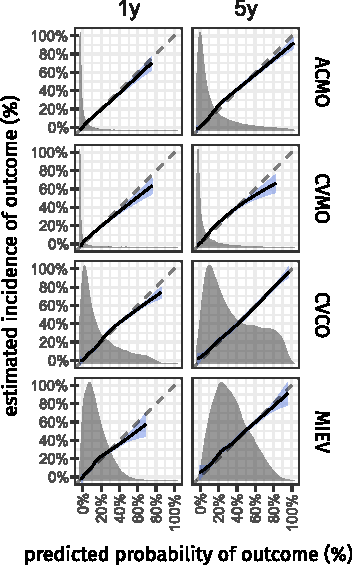
\includegraphics{graphics/pmhnet-v2-visual-calibration.pdf}
    \caption[Calibration of \pmhnet{2} models at 1 and 5 years]{%
        Calibration plots comparing 
        the cause-specific \(t\)-year \pmhnet{2} model predictions 
        with the estimated incidences at a 1 and 5 year prediction horizon.
        The included  regression line is obtained by fitting a natural
        cubic spline (\(d.o.f. = 6\)) with pseudo-values obtained
        by jackknife resampling of the Kaplan-Meier 
        (\acsfont{ACMO})
        or the Aalen-Johansen 
        (\acsfont{CVMO}, \acsfont{CVCO}, and \acsfont{MIEV})
        estimates.
        The dashed 45-degree reference lines represent perfect calibration. 
        The density curve in the background of each panel shows the 
        distribution of the model estimates.
    }
    \label{fig:pmhnet-v2-calibration}
\end{marginfigure}% ←

From visual inspection of the distribution of model predictions 
conditional on the observed outcomes (\cref{fig:pmhnet-v2-discrimination}),
we found the predicted cause-specific probabilities to be consistently higher 
for patients that experience the primary outcome (\enquote{primary})
compared to those that remained event-free (\enquote{event-free}).
This effect, however,  was less pronounced for the \acsfont{MIEV} 
outcome.
Interestingly, for the three outcomes with competing risks;
\acsfont{CVMO}, \acsfont{CVCO}, and \acsfont{MIEV};
the distribution of the primary-cause predictions
between patients experiencing the primary outcome (\enquote{primary})
and those experiencing the competing event (\enquote{competing}),
were overlapping considerably.
This suggests that it is difficult to distinguish between 
the competing risks, perhaps due to many shared risk factors,
indicating that treating competing events as censoring
would invalidate the assumption of uninformative censoring.

\begin{figure}[tpb]% →
    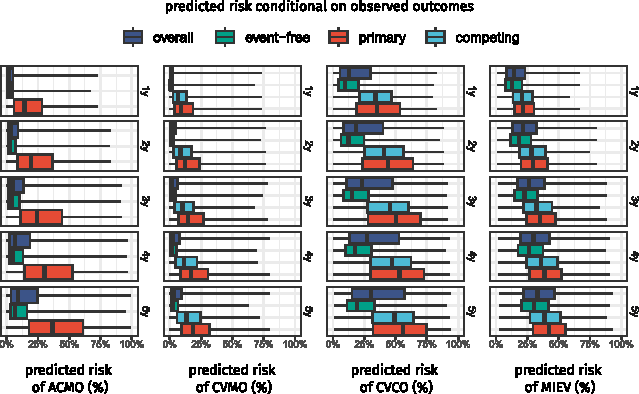
\includegraphics{graphics/pmhnet-v2-visual-discrimination.pdf}
    \caption[Test-set discrimination of \pmhnet{2}]{%
        Visual assessment of test set discrimination.  
        Boxplots display 
        the predicted \(t\)-year risk quantiles for the primary endpoints, 
        conditional on the observed \(t\)-year outcomes observed.  
        The boxplot marked \enquote{overall} show the observed 
        quantiles of the entire test set. 
        The quantiles included in the boxplots marked
        \enquote{primary}, \enquote{competing}, and \enquote{event-free}
        have been estimated using inverse probability of censoring weighting.
     }
    \label{fig:pmhnet-v2-discrimination}
\end{figure}% ←

To further quantify the model discrimination and calibration, 
we calculacted the \ac{tdAUC} and \ac{IPA} across 100 evenly separated
prediction horizons, ranging from 31 days to 5 years 
(\cref{fig:pmhnet-v2-performance}).
From this, we observed good model performance across
all tested prediction horizons.
For the three outcomes including competing risks,
we also included a naïve reference model where 
competing events were treated as censored.
We consistently found the \ac{tdAUC} and \ac{IPA}
of the naïve models to be worse than the competing-risk version.

\begin{figure}% →
    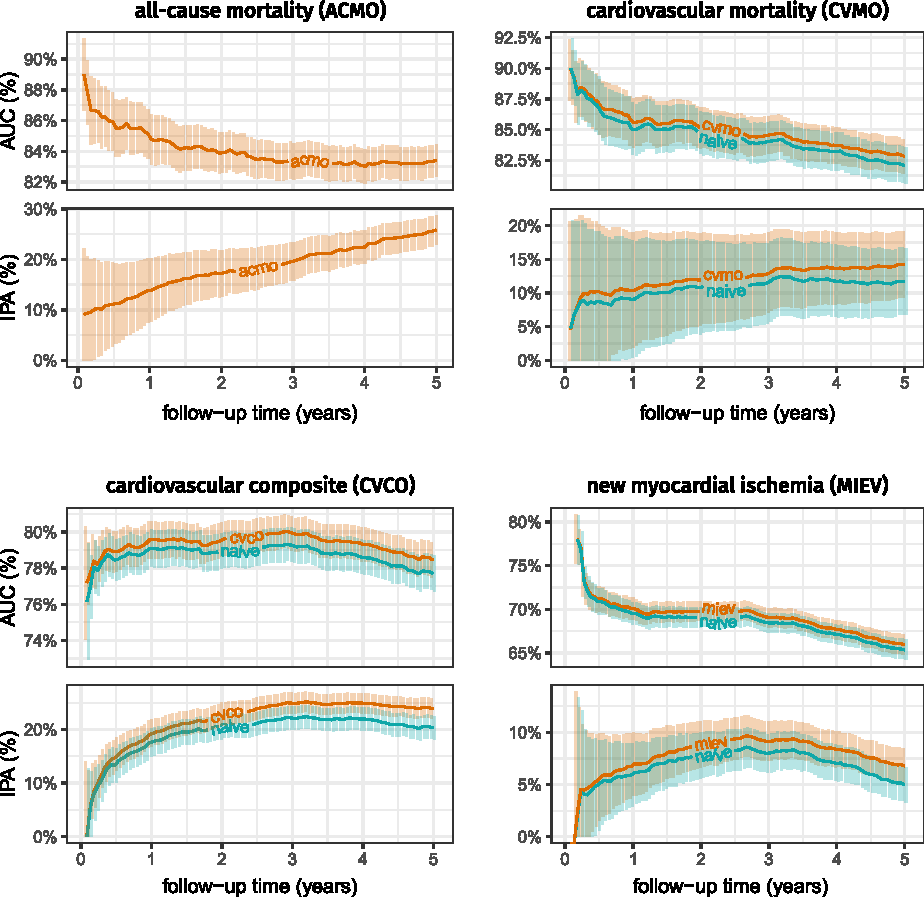
\includegraphics{graphics/pmhnet-v2-metrics.pdf}
    \caption[Test-set performance of \pmhnet{2}][-2em]{%
        \Acf{tdAUC} and \acf{IPA} for prediction of the primary
        endpoint for each of the four \pmhnet{2} models.
        \ac{tdAUC} and \ac{IPA} are computed at 100 evenly spaced
        timepoints, ranging from 31 days to 5 years.
        For the three outcomes including competing risks---%
        \acsfont{CVMO}, \acsfont{CVCO}, and \acsfont{MIEV}---%
        we also included a naïve single-risk model where 
        competing events were treated as censored.%
    }
    \label{fig:pmhnet-v2-performance}
\end{figure}% ←

To test the performance gain of jointly modelling the competing
risks, we analysed the differences in \ac{tdAUC} and Brier scores
between the competing-risk and the naïve versions across
the \acsfont{CVMO}, \acsfont{CVCO}, and \acsfont{MIEV} outcomes.
The results of these comparisons are summarised in \cref{tab:pmhnet-v2-delta},
which shows that in all cases, 
the competing risk models are better or 
comparable to models disregarding competing events.
Specifically, model calibration were found to be the most impacted
performance metric.

\begin{table}% →
    \small
\begin{tabularx}{\linewidth}{Xcccccc}\toprule
     & \multicolumn{3}{c}{ \(\Delta \mathrm{AUC}\)}
     & \multicolumn{3}{c}{ \(\Delta \mathrm{Brier}\)}\\
     \cmidrule(lr){2-4} \cmidrule(lr){5-7}

     & \multicolumn{2}{c}{ \(p < 0.05\)} & \(p \geq 0.05\)
     & \multicolumn{2}{c}{ \(p < 0.05\)} & \(p \geq 0.05\) \\
     \cmidrule(lr){2-3} \cmidrule(lr){4-4}
     \cmidrule(lr){5-6} \cmidrule(lr){7-7} 

     & \(\Delta > 0\) & \(\Delta < 0\) & \(\Delta \approx 0\) 
     & \(\Delta > 0\) & \(\Delta < 0\) & \(\Delta \approx 0\) \\
     \midrule

    \acsfont{CVMO} vs. naïve & 56 & 0 & 44 & 97 & 0 & 3 \\
    \acsfont{CVCO} vs. naïve & 91 & 0 & 9  & 97 & 0 & 3 \\
    \acsfont{MIEV} vs. naïve & 87 & 0 & 13 & 99 & 0 & 1 \\
    \bottomrule
\end{tabularx}
\caption[\pmhnet{2} performance gain by inclusion of competing risks]{%
    Differences in Brier score and \ac{tdAUC} 
    between the \pmhnet{2} competing risk models 
    and naïve reference models were competing events were treated as
    censoring. 
    The table shows the number of timepoints for which 
    the competing risk model had significantly better (\(\Delta > 0\)),
    significantly worse (\(\Delta < 0\)), 
    or comparable performance (\(\Delta \approx 0\))
    to the naïve model. }
\label{tab:pmhnet-v2-delta}
\end{table}% ←

\section{Conclusions}

In this study, we presented the development of \pmhnet{2}, 
an ensemble of four distinct neural network models for time-to-event 
prediction of important clinical outcomes in patients with \ac{IHD}.
These models were developed to predict the onset of important clinical
endpoints following coronary angiography:
all-cause mortality (\acsfont{ACMO}), 
cardiovascular mortality (\acsfont{CVMO}), 
cardiovascular complications (\acsfont{CVCO}), 
and new myocardial ischemia events (\acsfont{MIEV}). 

To enable the construction of these models, 
a central contribution of our research, 
is the development of a novel approach for
neural network-based modelling of 
discrete time-to-event data with competing risks.
This approach can be viewed as an extension to
Logistic-Hazard model from 
\textcite{gensheimerScalable2019},
and is grounded in classical statistical analysis of 
discrete time-to-event data.
~\autocite{tutzModeling2016}
To the best of our knowledge, 
we are the first to utilize this methodology
for neural network-based competing risk analysis.

Our approach has been implemented in the python package \texttt{DiscoTime},
a general-purpose software library that facilitates the application 
and further exploration of this methodology for 
time-to-event prediction with neural networks.
~\autocite{holmDiscotime}

In our experiments, \pmhnet{2} models,
utilizing this novel approach, 
provided accurate and well-calibrated time- and cause-specific 
estimates for secondary prognostication in patients with \ac{IHD}.
Compared to the common practice of treating competing events as censored,
our methodology demonstrated an increase in both model
discrimination and, particularly, in model calibration.
In the context of clinical research where competing risks are common,
this finding underscores the importance of using methodologies, 
like ours, that properly handle competing risks. 
Our study suggests such approaches should be considered in 
the development of future neural network-based medical risk prediction models.
 

\part{Concluding Remarks}
\chapter{Principal Findings, Limitations, and Future Perspectives}
\label{chap:findings-and-limitations}

In this thesis, I have explored the use of informatics-based approaches 
for addressing critical aspects pertinent to the understanding and management 
of \ac{IHD}. 
Central to this research was the application of advanced \ac{ML} methods
on large-scale electronic health data for development of precision medicine
approaches for secondary prevention in \ac{IHD}.
This involved identifying and characterizing patterns of multimorbidity 
in \ac{IHD} and developing feature-rich clinical prediction models for 
precision prognostication.

In this chapter, I will briefly reiterate the main findings of the 
included studies, adress some general and study-specific limitations
of the work undertaken, and discuss perspectives for future research.

\section{Principal Findings}

Throughout the previous chapters, 
I have described three different scientific manuscripts
detailing our research in the framework of \ac{ML}-based precision medicine.
The following provides a brief summary of the principal findings 
of each of the included studies.

\subsection{Comorbidity Clustering in Ischemic Heart Disease}

In \studyi{}, 
we used unsupervised clustering analysis to explore the comorbidity landscape
of \num{72249} patients with \ac{IHD}. 
We used the broadest possible definition of multimorbidity and 
defined comorbidity as the historical co-occurence of a broad
array of diagnosis codes in the individual patient records.
The accrued patient-specific comorbidity profiles,
containing more than \num{3000} different diagnosis codes,
led to the identification of 31 distinct patient subgroups.
These clusters represent distinct patterns of multimorbidity 
linked to \ac{IHD}, were found to be associated with 
specific risk of subsequent outcomes,
and can be used to better understand the complex
nature of multimorbidity in \ac{IHD}.

\subsection{Time-to-Event Prediction of All-Cause Mortality}

In \studyii{}, 
we presented the development and validation of 
a novel neural network-based prognostication model
for prediction of all-cause mortality in 
patients with \ac{IHD}.
This model, \pmhnet{1}, utilises a discrete-time approach 
for modelling of time-to-event data with neural networks and
can provide time-specific probability estimates of survival
across a five-year prediction horizon.
The model was developed using a large and diverse dataset 
\num{39746} \ac{IHD} patients from the \ac{EDHR}
and incorporates a comprehensive set of 584 features,
including diagnosis history, procedural codes, laboratory test results,
and clinical measurements obtained from \ac{EHR} data and registry data.
Compared to both the \acs{GRACE} 2.0 score, 
and a neural network-based model limited to the \acs{GRACE} features,
the feature-rich \pmhnet{1} model provided a significant improvement
in model performance.
External validation on an independent Icelandic dataset of \num{8287} patients 
further showed that the model performance is generalizable.
Furthermore, by including \acs{SHAP}-analysis we were able to provide
explanations of the model output and assess feature importance.
The study established \pmhnet{1} as a valuable tool for post-angiography 
assessment of all-cause mortality risk in \ac{IHD} patients,
and can potentially aid clinicians in making informed decisions 
about treatment and management of \ac{IHD}.

\subsection{Time-to-Event Prediction with Competing Risks}

In \studyiii{}, 
we introduced an new framework for construction of neural network-based
competing risk models and presented the development \pmhnet{2}, 
an advanced iteration of our \ac{IHD} prognostication algorithm.
The updated \pmhnet{2} model provide cause- and time-specific 
risk estimates for all-cause mortality, cardiovascular mortality, 
cardiovascular complications, and new myorcardial ischemia events.
From internal validation, we found the model estimates to
be well-calibrated and to accurately predict patient at 
both high and low risk of the four different outcomes.
Compared to the standard practice of treating competing events as 
censored, we showed that models capable of jointly modelling 
competing risks were associcated with a better model discrimination
and calibration.
While still a work in progress, the presented work establishes
the usefullness of the updated methodology and presents
\pmhnet{2} as a promising tool for prognostication in 
\ac{IHD}.

\section{Limitations}

Despite their strengths,
a number of limitations and constraints
related to the presented studies,
potentially affects the overall interpretation of the findings.
In the following,
I will address and discuss both study-specific
and general limitations of our research.

\subsection{Definition of Comorbidities}
\label{sec:comorbidities}

In \studyi{},
a possible limitation relates to its exclusively data-driven definition
of multimorbidity that included the historical co-occurence of a very broad 
array of diagnosis codes.
This approach constrasts with that of similar studies in the domain.
As an example, 
\textcite{formanMultimorbidity2018}
defined multimorbidity as
\textquote{two or more medical diseases or conditions, 
each lasting more than one year}. 
Similarly, another study also limited their definition
to only cover chronic conditions, specifically the 20 most
common ones.
\autocite{roccaPrevalence2014}
Unlike these studies that focused on chronic conditions,
our study did not differentiate between chronic and acute diagnoses. 
As a result, our clustering could, for example, 
be influenced by a 3-year old pneumonia diagnosis.
However, since we accrued the number of admissions for each diagnosis
the chronic nature of certain conditions is likely implicitly accounted.

\subsection{Lack of Temporal Resolution in Features}

In this thesis, a notable limitation is the absence of temporal resolution in
the input features, affecting both the clustering in \studyi{} and the
prediction models in \studyii{} and \studyiii{}. This lack of temporal
granularity means that the models and analyses do not account for the timing
and sequence of medical events or diagnoses.

In \studyi{}, the clustering could have been enhanced by somehow 
incorporating the chronological order of the diagnoses in the patient vectors.
This would allow for a more nuanced description of the comorbidity burden
of the individual patient, and could in addition help alleviate the limitation
of chronic versus acute conditions described in \cref{sec:comorbidities}.
Previous research within our group by \textcite{jensenTemporal2014} illustrated
a method to identify temporal disease trajectories from retrospective registry
data. They also demonstrated the use of these trajectories in clustering
applications. However, this method only captures temporal patterns with clear
directionality, which could exclude many of the comorbidities we considered in
our study. Thus, while it offers a possible avenue for future research,
it also has its limitations in fully representing the range of
comorbidities.

In \studyii{} and \studyiii{}, time resolved input features could enable 
the neural network models to learn from sequential patterns of medical
events and diagnoses. Such information could provide valuable information
for accurate prognostication. For instance, knowing the progression of 
\ac{IHD} and comorbidities could potentially inform more timely and tailored
interventions. Additionally, the study design used in the development of
\pmhnet{1} and \pmhnet{2} was limited in scope to only provide predictions
subsequent to an index coronary angiography. While these models 
might be applicable at other timepoints, it is not something that we have tested,
and it would probably affect their performance.

Alternatives to address this limitation include the use of time-series data 
and longitudinal study designs such as those based on landmark analysis.
\autocite{dafniLandmark2011}
These approaches can facilitate the creation of dynamic risk prediction
models.
\autocite{vanhouwelingenDynamic2007}
In the context of neural networks, this would likely involve
using architectures like 
\ac{LSTM}~\autocite{hochreiterLong1997}
or Transformers~\autocite{vaswaniAttention2017},
which are designed to use sequential features.

\subsection{Generalisability of Clusterings}

For \studyi{},
an inherent limitation of clustering applications is 
the lack of standardized techniques for external \enquote{validation}
compared to those in supervised learning.
In supervised learning, 
evaluating the model generalizability is straightforward:
apply the model to a test set, 
which could be an internal hold-out set or an external dataset,
and then directly measure its performance.
However, this approach is not feasible in most unsupervised clustering
applications due to the absence of predefined labels.
Alternative strategies do exists,
as outlined by \textcite{ullmannValidation2022},
and includes:
\begin{itemize}
    \item Applying the clustering algorithm to a representative external
        dataset. Subsequently, examine if the cluster structure obtained on
        this external dataset shares internal and external characteristics with
        the original clustering. 
    \item Transferring the original clustering to the external dataset by first
        using, for example, a supervised classifier. 
        ~\autocite{ullmannValidation2022}
        This classifier is trained to predict
        the cluster labels derived from the original dataset and then applied
        to the external dataset. 
        If clustering on the external data is consistent with the transferred
        labels, then it indicates that the cluster algorithm have 
        captured patterns that are not just specific to the initial
        dataset.
\end{itemize}

Such approaches, while not direct validations in the traditional sense, 
could provide insights into the overall generalisability of the clustering 
outside the context of the original dataset.
~\autocite{ullmannValidation2022}
Nonetheless, these approaches have not been implemented in our research.
Consequently, we do not assert that the clustering presented is definitively
the \enquote{best} but rather utilize it as a method to condense the extensive
array of diagnostic codes into interpretable subgroups.

\subsection{Choice of Clustering Algorithm}

A further potential limitation of \studyi{} 
is that we did not compare or test other 
clustering methodologies besides the \ac{MCL} algorithm.
Although numerous different clustering algorithms exists,
our choice of using \ac{MCL} was motivated by a number of key aspects.
Firstly, the \ac{MCL} algorithm is fast and has been explicitly designed 
to handle very large networks with a substantial number of vertices
and edges.
~\autocite{vandongenGraph2008}
Secondly, in this algorithm,
the number of clusters neither can nor should be pre-specified.
Instead the issue of \enquote{how many clusters} is handled
by a strong internal logic, rather than being dealt with in an
arbitrary manner as is common in other clustering algorithms.
~\autocite{vandongenGraph2008}

\subsection{Lack of Primary Care Data}

A fundamental limitation in our research stems from the nature of the data
accessed, as all our studies primarily utilized hospital data. This
reliance on hospital data is likely to lead to an underrepresentation 
of data related to conditions and diseases primarily managed in primary
care settings, including hypertension, non-complex infections, and various
soft-tissue disorders.
~\autocite{finleyWhat2018} 

In \studyiii{}, we attempted to mitigate this limitation by incorporating
prescription data, which can serve as proxy for the conditions managed
in primary care.
However, it is important to note that prescription data is only partly
able to compensate for the lack of detailed primary care patient records.

\subsection{Limitations of Explainable AI}

The last limitation I would like to higlight are some general shortcomings
of \ac{XAI} that often are overlooked. Currently, \ac{XAI} is only implemented
in \studyii{}, but our plan is include it in \studyiii{} as well, and for 
this future work, these limitations also apply.

As described earlier in this thesis, 
the goal of \ac{ML} is to make accurate predictions on unseen data,
and as consequence, the \enquote{how} and \enquote{why} of predictions
is of less concern.
However, for critical applications, including healthcare, it is 
generally agreed that transparency is important and that 
the \enquote{black box} nature of \ac{ML} needs to be 
adressed. 
~\autocite{topolHighperformance2019}
This is exemplifed by article 15,
of the European Union's \ac{GDPR},
~\autocite{EuropeanParliament2016a}
which specifies an requirement for transparency that 
applies to algorithmic decision-making.%
\sidenote{%→
    Item (h) in paragraph 1 of the \acs{GDPR} article 15 states that
    \textquote{%
     the existence of automated decision-making, including profiling, referred to
     in Article 22(1) and (4) and, at least in those cases, meaningful information
     about the logic involved, as well as the significance and the envisaged
     consequences of such processing for the data subject.}%
}% ←

For \ac{ML}, including neural networks, \ac{XAI} is a form of post-hoc
analysis that seeks to provide the required transparency for 
otherwise complex and non-transparent models.
In this domain, \acsu{SHAP}-analysis~\autocite{lundbergUnified2017},
which we utilized in \studyii{} 
for providing explanations of the \pmhnet{1} model,
is arguably one of the most popular \ac{XAI} approaches.
\ac{SHAP},
along with other similar approaches,
relies on the usage of simpler surrogate model
to estimate the expected marginal contribution
of each feature to the model's output.
~\autocite{bellePrinciples2021}
However, this approach requires certain assumptions,
including the premise that the model can be locally
approximated by a simpler model and that features
are independent.
~\autocite{lundbergUnified2017}
The independence assumptions is very strong and often very unrealistic,
which is likely to bias the estimates of feature contributions---%
nevertheless, this approach is still in widespread use.
Recent research has demonstrated that is is possible to partially mitigate
this limitation, but at the expense of a significantly increased computational
complexity, which can limit its practical usefulness.
\autocite{aasExplaining2021}

\ac{XAI} algorithms such as \ac{SHAP} are approximations 
of the complete model, therefore the fidelity is not perfect
and as a consequence, neither are the explanations.
Currently, there are no established standards for assessing the quality
of these explanations.
While it is possible the esimate the error of the approximations,
this does not necessarily indicate whether the explanations are interpretable
and understandable to end-users. 

From a practical standpoint,
the explanations offered by \ac{XAI} can be subject to misinterpretation,
particularly by users less familiar with technical details of 
the \acsu{AI}-model and the \ac{XAI} method used.
During the clinical implementation of the \pmhnet{1} model for a, 
currently ongoing, clinical trial~\autocite{bundgaardClinical2023}, 
we provide \ac{SHAP} values alongside the model predictions to inform 
clinicians on the basis of the model predictions.
However, a pilot experiment in which clinicians were asked to qualitatively 
evaluate the model's output and explanations revealed some challenges in 
the interpretation of these.

For example, one clinician found it counterintuitive that the model identified
hyperlipidemia (\acs{ICD-10}: E78) as a factor contributing to increased 
survival.
While it is possible that this finding is caused by the aforementioned
limitations, there are other plausible explanations as to why
hyperlipidemia could be identified as a \enquote{protective} feature.
It is important to note that \ac{SHAP} values are correlations and 
do not imply causation.
Patients already known with hyperlipidemia prior to
their index coronary angiography may represent a 
group of patients with non-acute manifestations of \ac{IHD},
which relative to the median \ac{IHD} patient could
have improved survival.
Additionally, these patients are likely to have
initiated statin treatment before the time of prediction,
which once again, could be associated with a improved
prognosis relative to the median patient.

This example underscores the complexities inherent in
interpreting \ac{XAI} explanations, especially when they appear
counterintuitive or misaligned with conventional medical knowledge. 
It also emphasizes the need for thorough education and effective communication
with healthcare professionals regarding clinical decision support tools that
incorporate these technologies.

\section{Future Perspectives}

Adressing the various just discussed limitations and constraints
all represent topics for future research, some more important than others.
To conclude this thesis, I would like to highlight two central challenges
related to this thesis project of utmost importance for future data-driven 
research in precision medicine.

\subsection{Clinical Implementation of Machine Learning Models}

In this thesis, I have argued for the potential benefits of \acsfont{AI/ML}
methodologies in improving the clinical treatment and management of patients
with \ac{IHD}. We have developed two neural network-based \ac{IHD}
prognostication models, evaluated their performance using state-of-the-art
statistical metrics, and concluded that high-dimensional \ac{ML}-based
models are superior to existing alternatives.
However, the theoretical clinical impact is, as of now, only just that---%
theoretical. 

It is generally accepted that
the overwhelming majority of published medical prediction models 
are never implemented in clinical practice.
~\autocite{steyerbergPrognosis2013}
To increase the adoption of \ac{ML}-based prognostic models, 
we need more prospective clinical studies to ascertain 
the impact and practical applicability of such models.
This includes exploring how \acsfont{AI/ML} can positively   
affect clinical decision-making, patient outcomes, and 
allocation of healthcare resources.
Such research is crucial in realising the potential of 
\acsfont{AI/ML} in the advancement of precision medicine.

As an extension of the work presented in \studyii{},
although not included as a central part of this thesis,
we have established a collaboration with the public company 
\acsfont{CIMT} to implement \pmhnet{1} in \enquote{Sundhedsplatformen}, 
the \ac{EHR} system used in the Capital Region and Region Zealand hospitals,
for prospective clinical validation.
We successfully integrated the model into a real-world clinical \ac{EHR}
setting and have initiated a clinical trial.
~\autocite{bundgaardClinical2023} This study is still in progress, but
independently of its outcomes, the mere implementation of the model in a
clinical setting is a significant achievement.

Looking ahead, depending on the findings of this trial,
the focus needs to shift towards the implementation of processes
for continuous monitoring of model performance, for regularly updating
the model with new data, for refining models to include additional 
endpoints (\pmhnet{2}), and several other important aspects.

\subsection{Sharing of Healthcare Data}

As outlined in \cref{chap:data-foundation}, 
the studies presented in this thesis draws on hospital data from 
more than \num{2.6} million individuals, which originates from
combination of different data sources, including
electronic health records, national registries, 
and clinical quality databases.
In the context of this thesis project,
a major challenge have been
processing, combinining, cleaning, and 
organizing these diverse sources of data
into curated datasets appropriate for 
\ac{ML} applications.

However, because such data, for good reason, is subject to ethical 
and privacy-protecting rules and regulations, it cannot realistically 
be shared with researchers outside our institution.
This means that it is impossible for others to reproduce our findings,
develop and benchmark rival models, and benefit from the data cleaning
and curation that have already been done.
It is a waste of resources and limits the development of the field as a whole.

It is evident that 
there exists an unmet need for regulations and approaches that enable 
combining and benefitting from otherwise siloed datasets.
In this context,
the concept of federated health data networks have been 
suggested as a possible solution to overcome existing barriers preventing 
sharing of data.
~\autocite{hallockFederated2021}
In the ongoing effort of establishing a European Health Data Space, 
the European Commission's proposal have also included procedures and
regulations for secondary research use of health data.
As suggested by \textcite{raabFederated2023}, 
this effort could be coupled with the establishment of
pan-European federated health data network, which could break
the many barriers limiting current big data-based clinical research.

Future research should focus on technical solutions for 
establishing such networks, development of algorithms for 
distributed machine learning, and construction of interoperability 
formats which could further cross-institutional and international 
collaboration.
      

\backmatter %%%%%%%%%%%%%%%%%%%%%%%%%%%%%%%%%%%%%%%%%%%%%%%%%%%%%%%%%%%%%%%%%%%

\bookmarksetup{startatroot}
\addcontentsline{toc}{chapter}{List of References}
\printbibliography

\mainmatter %%%%%%%%%%%%%%%%%%%%%%%%%%%%%%%%%%%%%%%%%%%%%%%%%%%%%%%%%%%%%%%%%%%

\appendix
\appendixpage
\addappheadtotoc
\cleardoublepage

\includepdf[
    clip, trim=1cm 6cm 1cm 1.8cm, offset=0 -2.2cm, 
    frame=true, scale=0.8, pages=1, 
    pagecommand=\chapter{Manuscript for Study I}\label{chap:study1-paper}]%
    {assets/paper1-clustering.pdf}

\includepdf[
    clip, trim=1cm .5cm 1cm 1.6cm, offset=0 0, 
    frame=true, scale=0.8, 
    pages=2-5, pagecommand={}]%
    {assets/paper1-clustering.pdf}

\cleardoublepage
\includepdf[
    clip, trim=1cm 4cm 1cm 4cm, offset=0 -2.2cm, 
    frame=true, scale=0.8, pages=1, 
    pagecommand=\chapter{Manuscript for Study II}\label{chap:study2-paper}]%
    {assets/paper2-pmhnet-v1.pdf}

\includepdf[
    clip, trim=1cm 2cm 1cm 3.2cm, offset=0 0, 
    frame=true, scale=0.8, pages=2-5, 
    pagecommand={}]%
    {assets/paper2-pmhnet-v1.pdf}

\cleardoublepage
\includepdf[
    clip, trim=1cm 8cm 1cm 2cm, offset=0 -2cm, 
    frame=true, scale=0.8, pages=1, 
    pagecommand=\chapter{Manuscript for Study III}\label{chap:study3-paper}]%
    {assets/paper3-pmhnet-v2.pdf}

\includepdf[
    clip, trim=1cm 1.4cm 1cm 1.8cm, offset=0 0, 
    frame=true, scale=0.8, pages=2-5, 
    pagecommand={}]%
    {assets/paper3-pmhnet-v2.pdf}

\end{document}
